%%% Local Variables: 
%%% mode: latex
%%% TeX-master: t
%%% End: 

\documentclass[a4paper,adobefonts,cs4size,fancyhdr,fntef]{ctexrep}
\usepackage{amsmath,amssymb,algorithm,algorithmic,booktabs,graphicx,paralist,supertabular,subfig,metalogo,mflogo,texnames,listings}
\newcommand{\thesistitle}{电流表读数自动识别} %论文标题
\graphicspath{{scu/}{mask/}{process/}} %设置插图目录
\renewcommand{\emph}[1]{\textit{#1}} %fntef选项改变了\emph命令的定义,我再改回来
\renewcommand{\CJKunderlinecolor}{\color{black}} %fntef宏包默认下划线为蓝色,改成黑色
%将版面大小和位置为和Word的默认版面相同。注意,Word的默认版面的有关参数均以英寸(inch)作单位,不是以厘米(cm)作单位。毕业论文模板给出的参数都是错的。连Word都不熟,还好意思做模板。
\usepackage[left=2.5cm,right=2cm,top=2.8cm,bottom=2.8cm]{geometry}
%设置图表标题样式
\usepackage{caption}
\DeclareCaptionFont{hei}{\heiti\zihao{5}}
\captionsetup{font=hei,labelsep=quad}
% 定公式、图、表编号为"3-1"的形式,即分隔符由.变为短杠
\renewcommand\theequation{\arabic{chapter}--\arabic{equation}}
\renewcommand\thefigure{\arabic{chapter}--\arabic{figure}}
\renewcommand\thetable{\arabic{chapter}--\arabic{table}}

%设置章节标题样式。不知道是哪个二货想出的这么难看的样式,不用Word或LaTeX默认的样式会死啊。
\CTEXsetup[name={,},number={\arabic{chapter}},format={\zihao{-3}\centering},beforeskip={-35pt},afterskip={15pt plus 2pt minus 2pt}]{chapter}
\CTEXsetup[format={\zihao{4}\bf\flushleft},beforeskip=12pt,afterskip=12pt]{section}
\CTEXsetup[format={\zihao{-4}\heiti\flushleft},beforeskip=10pt,afterskip=10pt]{subsection}
\CTEXsetup[format={\zihao{-4}\heiti\flushleft},beforeskip=10pt,afterskip=10pt]{subsubsection}
\CTEXsetup[number={\arabic{chapter}}]{appendix} %附录用数字编号
%设置页眉页脚
\pagestyle{fancy}
\fancyhf{}
\fancyhead[L]{\small\bf 四川大学本科毕业论文}
\fancyhead[R]{\small\bf \thesistitle}
\fancyfoot[C]{\thepage} %奇数页的页眉和偶数页的一样,而奇数页的页码和偶数页的页码却是对称摆放。在一般的文献中,页眉页脚要么都对称,要么都一样。再次证明模板的作者是一位完全不懂排版的二货。

%在默认情况下,每一章第一页的页眉不显示,而模板要求显示,所以给这一页加页眉。
\fancypagestyle{plain}
{
  \fancyhf{}
  \fancyhead[L]{\small\bf 四川大学本科毕业论文}
  \fancyhead[R]{\small\bf \thesistitle}
  \fancyfoot[C]{\thepage}
}
\floatname{algorithm}{算法} %将算法标题的标志Algorithm改为“算法”
\renewcommand{\algorithmicrequire}{\textbf{输入}} %把算法的Require改为“输入”
\renewcommand{\algorithmicensure}{\textbf{输出}} %把算法的Ensure改为“输出”
%自定义一组函数。在数学模式下,函数的字体为直立罗马体,变量的字体为斜体。
\DeclareMathOperator{\search}{search}
\DeclareMathOperator{\neighbours}{neighbours}
\DeclareMathOperator{\make}{make}
\DeclareMathOperator{\union}{union}
\DeclareMathOperator{\find}{find}
\DeclareMathOperator{\labelset}{labelset}

%定义GBT7714-2005N标准的参考文献样式
% \usepackage[super,square,numbers,sort&compress]{natbib}
% \bibliographystyle{GBT7714-2005NLang}
\newcommand{\upcite}[1]{\textsuperscript{\cite{#1}}} %将参考文献数字列到右上角
%\usepackage[CJKbookmarks,colorlinks,linkcolor=blue,bookmarks=true,pdfpagemode=UseOutlines,pdfauthor={何为},pdfsubject={数字图像模式识别},pdftitle={\thesistitle},pdfkeywords={图像处理,字符识别}]{hyperref} %hyperref包容易和其他宏包冲突,所以放在最后
\begin{document}
\begin{titlepage}
\renewcommand{\CJKunderlinecolor}{\color{black}}
\newcommand{\titleterm}[2]{\makebox[4em][s]{#1}\CJKunderline{\makebox[14em]{\kaishu #2}}}
\begin{center}
\includegraphics[scale=0.5]{name.eps}\\[10pt]
\songti\zihao{1} 本科生毕业论文(设计)\\[10pt]

\includegraphics[scale=0.3]{brand.eps}\\[10pt]
\songti\zihao{4}
\baselineskip=1.5\baselineskip
\titleterm{题目}{\thesistitle}\\
\titleterm{学院}{计算机学院}\\
\titleterm{专业}{计算机科学与技术}\\
\titleterm{学生姓名}{何为}\\
\makebox[4em][s]{学号}\CJKunderline{\makebox[7em]{0943041105}}年级\CJKunderline{\makebox[5em]{\kaishu 2009级}}\\
\titleterm{指导教师}{张蕾}\\[1ex]


教务处制表\\
二ΟΟ八年六月一日
\end{center}
\end{titlepage}

%%% Local Variables: 
%%% mode: latex
%%% TeX-master: "thesis"
%%% End: 
 %封面页
\begin{center}
\vspace*{18pt}
{\heiti\zihao{-2}\thesistitle}\\[18pt]
\zihao{4}{\kaishu 专业名称}\quad 计算机科学与技术\\[12pt]
{\kaishu 学生} \quad 何为 \quad {\kaishu 指导老师} \quad 张蕾\\[24pt]
\end{center}\par

\zihao{5}[{\heiti摘要}]
自动处理和识别图像是一个重要的领域。近几十年来,随着计算机的存储和运算能力的提高,制约图像处理和机器视觉技术应用的障碍逐渐减少,图像处理和机器视觉技术在实际生产生活中得到了广泛的应用。在航空遥感、车牌识别、医学图像、安全防卫、工业制造等领域,都有图像处理和机器视觉技术的应用。例如在制造业中,机器视觉技术常用于检测产品质量。在门禁系统中,可以用图像处理技术识别人脸,确定身份。在图书馆和档案馆,扫描纸质文档后,常用图像识别技术识别文本,以文本而非图片的形式存储文档。

某电站有许多半机械式的电流表。由于电流表数量多,位置分散,且工作在高压环境中,人工抄表费时费力,又有较大的危险。虽然已有电子式电流表,但这些电流表体积庞大,且距离高压线较近,拆卸极为不便且危险。再加上人工抄表的办法难以实现电流的实时监控。综合上述原因,为进行实时监控并减少工作量,在电流表前安装摄像头,从采集的图像中识别电流表读数,是一个可行的办法。

通过摄像头采集电流表图像得到电流表的彩色图像。其中数字只占很小的一部分,而且被周围复杂的区域包围,对读数识别造成干扰。因此分离与数字无关的区域,准确提取数字,直接关系到识别率的高低。针对这种情况,本文将读数识别分成通过图像预处理、数字边框提取、数字分割和数字识别这四个过程。其中前三个步骤均用于消除噪声和排除无关区域。在预处理过程中,首先将摄像头拍摄的彩色图像转换成灰度图像。由于图像含有较多噪声,而且部分图像偏亮或偏暗,所以进行高斯滤波和直方图均衡化处理。在数字边框提取的过程中,首先根据灰度图像中黑色和白色区域面积较大的特点,选用Otsu阈值法得到二值化的图像。二值化的图像包含边框的若干候选区域,用连通成分标记算法从中找出数字边框。由于数字边框有一定的倾斜,用哈夫变换找出倾斜角,然后旋转图像。在字符分割部分,本文使用基于阈值的分割算法。首先用阈值法分割图像,然后做水平和竖直方向的投影,找出每个数字的位置。最后在字符识别的过程中,针对多个电流表的数字形状一致,分割出的数字有部分缺失的情况,提出用模板匹配法识别字符。实验表明,上述方法取得了较好的识别效果。

\vspace{10pt}

[{\heiti 主题词}]{\kaishu 电流表;\quad 图像分割;\quad 字符识别}

%%% Local Variables: 
%%% mode: latex
%%% TeX-master: "thesis"
%%% End: 
 %中文摘要
\begin{center}
\vspace*{12pt}
{\bf\zihao{-2}Automatic Ammeter Digit Recognition}\\[18pt]
\zihao{4}Computer Science and Technology\\[12pt]
{\bf Student} \quad Wei HE \quad {\bf Advisor} \quad Lei ZHANG\\[24pt]
\end{center}\par

{\zihao{5}[{\bf Abstract}] Automatic image processing and recognition is an important field. In recent decades, as the storages volumn and computation speed of computers have been considerably improved, the obstacles that once prevented the application of image processing and computer vision no longer exist. Because of this, Image processing and computer vision has been widely employed in plate number recognition, medical image processing, security and manufacturing. For instance, in manufacturing, computer vision is often used to inspect the defects of products. In , image processing is used to recognise the identity of guests. In libraries and archieves, printed essays are scanned and their texts are automatically recognised.

There are many semi-mechanical ammeters in a power station. Due to the fact that these ammeters are scattered and located in high voltage environment, it is arduous and hazardous for workers to read the meters. These semi-machanical ammeters cannot be replaced by electronic ammters in short period, as they are considerably large and installed in cabinet tightly. Because of this, in order to reduce the workload and achieve real-time monitoring, it's essential to recognise the digits in the images of them.

The cameras in front of them capture color image. The digits in the images takes only a small part, which is surrounded by several areas, causing interference in recognition. Therefore, it is a key point to separate digits and other parts. Considering these facts, the thesis propose  be divided into four stages consequently: preprocessing, frame positioning, digit seperation and digit recognition. During preprocessing stage, the color image is converted to gray-scale image at first. After that, we perform Gaussian blur and histogram equalization. During the stage of frame positioning, we can use Otsu algorithm to acquire binary image. Then we use connected components labeling algorithms to find out the frame. Since the frame is slanted, we apply Hough transform to determine the slope and calibrate the frame. In the segmentation stage, the thesis proposes a threshold based segmenting algorithm. After that, projections on both horizontal and vertical axis are performed to locate the digits in images. In the last stage, as the digits in ammeters are consistent, the thesis propose template matching algorithm to recognise the them. The experiments have proved the effect of the algorithms.
}

\vspace{10pt}

[{\bf Key Words}]{Ammeter, Image Segmentation, Charactor Recognition}

%%% Local Variables: 
%%% mode: latex
%%% TeX-master: "thesis"
%%% End: 

 %英文摘要
\zihao{-4}
\tableofcontents

\chapter{绪论}\pagenumbering{arabic}

\section{课题的背景}

各种各样的仪表用于测量系统,其中大多数仪表是机械式和半机械式的。这些仪表不能以数字化的形式存储读数,也没有数据接口传输读数。这些仪表的读数需要人工抄录。在有些场合下,人工抄录是可行的。但在另一些场合下,人工抄录不能满足要求。在需要实时监控的场合,用人工抄录的办法不能及时使响应读数的异常变化,也很难做到全天24小时监控。在化工、钢铁、冶金和核辐射等危险场合,人工读数威胁到工作人员的安全,是不现实的做法。

随着图像处理、模式识别和机器视觉等技术的发展,许多图像识别任务都可以使用计算机自动完成。例如在制造业中,常常利用机器视觉方法自动地检测产品的质量,从而极大地提高生产的自动化程度;在海关、自动柜员机、门禁系统中,通过扫描虹膜或人眼,计算机系统能识别身份;在银行业,机器视觉方法用于自动地识别印章真伪;档案管理系统也可以用机器视觉技术将纸质文档数字化,以便于存储和检索。仪表读数识别也可以利用机器视觉技术完成。通过自动识别仪表读数,可以方便地进行集中管理,及时地对异常情况进行处理。



\section{课题的意义}

本文要识别的电流表来自于发电厂。这些电流表都是半机械式的。由于电流表在高压环境中,人工抄表有较大危险。另一方面,这些电流表体积庞大,且安装在整套的仪表柜中,很难取出,这些半机械式的电流表暂时无法替换成电子式电流表。为了实现实时监控,可以在电流表前安装摄像头,实时采集电流表图像,然后用计算机系统识别。这种方式能减少工作量,实现无人值守的电流监控。随着电子技术和计算机技术的发展,各种图像采集系统和机器识别系统的性能越來越高,价格也具有很强的竞争力。因此,用仪表读数的自动识别代替人工抄表,能降低人力成本,也可以减少高电压的危险环境对工作人员的伤害。

%基于机器视觉的远程仪表自动抄表系统的出现将极大地提高抄表的速度和准确率性,进而提高工作效率,降低企业经营成本,同时对于这些特定的危险环境,可以减少对人的伤害。通过齿轮来显示表盘数字的仪表在读取的过程中有着相似的显示规律,因此基于机器视觉的仪表数字识别研究在某些特定的实际生产生活中有着非常广阔的应用前景。

电流表的仪表读数识别技术也可以推广到其他仪表的读数识别。部分仪表由于其工作原理和测量环境的特殊性,不宜安装电子线路,如油位计、流量计和气表等,为了实现自动抄表,采集这些仪表的图像进行读数识别是一个可行的选择。在核电站和化工厂等危险场所,如果进行人工抄表,工作人员可能受到较大的伤害。利用机器视觉技术实现远程抄表,可以减少对工作人员的危害。对仪表实现自动读数后,与计算机系统连接,实现管控自动化,进而提高工作效率,降低管理成本。

\section{相关工作}

仪表读数识别涉及数字图像处理技术。随着计算机的计算速度和存储能力的迅速发展,图像处理所需的极高的计算和存储要求得到满足。限制图像处理技术应用的因素大多被消除。 数字图像处理技术得到广泛应用。

仪表读数识别和光学字符识别有着很紧密的联系。早在1929年,德国就出现了第一份有关光学字符识别的专利\upcite{compvision}。到五十年代计算机出现时,IBM公司便开始光学字符识别的研究,当时用于扫描美国政府浩如烟海的纸质档案,以文本的形式储存在计算机中\upcite{machvision}。从八十年代开始,CCD和CMOS等图像采集器件和大规模集成电路的出现,使数字图像的采集、存储和处理技术跃上了一个新的台阶,光学字符识别技术也随之得到极大的发展。光学字符识别技术用于档案扫描、信件分拣、车牌识别等方面。特别值得一提的是由惠普研究院研制的tesseract-ocr软件\upcite{tes}。它能读入多种格式的图像,并能识别超过60种语言的文本图像。在光学字符识别精度的竞赛中,它也名列前茅。

我国在数字识别方面的研究从八十年代开始,起步比国外晚\upcite{meter1}。几十年来,科研人员付出了艰辛的劳动,取得了丰硕的成果。光学字符识别技术取得了长足的进步。如今,对于常见的光学字符应用,已经有了成熟的解决方案。在交通领域,光学字符技术广泛地用于车牌识别\upcite{meter1}。在印刷体字符识别领域,由清华大学研发的TH-OCR获得了业界广泛的认可\upcite{machmeter}。目前,光学字符识别理论非常成熟,对于较清晰的字符,识别率已接近100\%\upcite{vcimg},这些为仪表读数的计算机识别奠定了坚实的基础。

%%% Local Variables: 
%%% mode: latex
%%% TeX-master: "thesis"
%%% End: 


\chapter{图像处理基本理论}

\section{图像增强}

实际图像不是完美的。由于噪声和光照等原因,图像的质量达不到自动识别的要求,所以需要进行图像增强\upcite{img_process}。图像增强可以突出待识别的目标的特征,抑制噪声和目标外的部分,从而使增强的图像更适合计算机识别。常见的图像增强方法有\emph{灰度变换}和\emph{图像平滑}。

\subsection{灰度变换}

灰度变换就是将图像每个像素的灰度变换成另一种灰度。灰度变换后每个像素的灰度仅仅由变换前的灰度决定。如果输入图像为$F(i,j)$,输出图像为$G(i,j)$,则灰度变换可以表示为:
\begin{equation}
  G(i,j)=T(F(i,j))
\end{equation}
变换函数$T(x)$可以由用户指定,也可以根据直方图确定。\emph{直方图均衡}就是一种根据直方图确定变换函数的方法。直方图均衡主要用于增加图像的全局对比度,改善光照条件不佳的图像。例如对背景或前景过亮或过暗的图像进行光照补偿,增强曝光过度或曝光不足的图像的细节等。直方图均衡化使输出图像包括所有可能的灰度级,并在每个灰度级上有大致相等的像素个数。要达到上述要求,首先求出直方图。设$n$表示图像的像素数,$n_i$表示灰度$i$出现的次数。灰度$i$有$0,1,\cdots,L-1$共$L$个灰度级。则直方图均衡化的灰度变换函数$T(x)$可以用如下方式求出。直方图$p(i)$表示灰度$i$出现的概率,用公式表示为:
\begin{equation}
  \label{eq:hist}
  p(i)=\frac{n_i}{n},i=0,1,\cdots,L-1
\end{equation}
再从直方图求出累计概率函数$c(i)$,定义如下:
\begin{equation}
  \label{eq:acc}
  c(i)=\sum_{j=0}^i p(j)
\end{equation}
最后将$c(i)$映射到$L$个灰度级:
\begin{equation}
  \label{eq:map}
  m(c(i))=\left[\frac{c(i)-\min(c(i))}{\max(c(i))-\min(c(i))}\cdot L\right]
\end{equation}
此时得到灰度变换函数为$T(x)=m(c(x))$。

\subsection{图像平滑滤波}

原始图像一般含有较多的噪声。噪声一般表现为盐椒噪声或孤立的点线噪声。图像平滑滤波使图像模糊化,去除极小的细节或将图像内的小间断连接起来。图像平滑滤波的基本方法是在像素的邻域内,对邻域内的像素和对应的系数的乘积求和。邻域内像素位置对应的权值一般用\emph{表示}。用模板进行图像滤波的方法如下:
\begin{asparaenum}[(1)]
\item 将模板中心与某个像素重合;
\item\label{enum:mul} 将模板上的权值和模板下对应的像素值相乘;
\item\label{enum:sum} 将第(\ref{enum:mul})所得的所有乘积相加;
\item 将模板中心的像素的灰度值用第(\ref{enum:sum})步的结果代替。
\end{asparaenum}


\emph{盒形滤波}是最简单的平滑滤波方法。它将每个像素的灰度用其邻域的算术平均值代替。设$F(i,j)$表示输入图像,$G(i,j)$表示平滑的图像,$S$表示邻域的像素坐标集合,$M$表示邻域的像素数目,则盒形滤波可以用公式表示为
\begin{equation}
  G(i,j)=\frac{1}{M}\sum_{(m,n)\in S}F(m,n)
\end{equation}
盒形滤波的模板如图\ref{fig:box}所示。
\begin{figure}[!h]
  \centering
  \includegraphics{box.eps}
  \caption{盒形滤波的模板}
  \label{fig:box}
\end{figure}

\emph{高斯滤波}也是一种常见的图像平滑滤波器。高斯滤波的模板对距离中心越远的位置,取越小的权值。与盒形滤波模板相比,高斯滤波更适合消除高斯噪声。这是因为空间域的高斯函数的傅立叶变换是频率域的另一个高斯函数,说明进行高斯滤波时,空间域内噪声对应的高频部分的衰减程度比低频部分大,噪声得到较大的抑制。高斯滤波对边缘的影响比盒形滤波小。这是因为图像的边缘中心像素和周围像素反差较大。应用盒形滤波时,由于模板对边缘中心和周围像素取相同的权值,边缘和周围区域的反差减小,不利于边缘检测。而对边缘应用高斯滤波时,模板中心的权值比周围像素的权值大,边缘和周围区域的反差减小的幅度较低,对边缘检测的影响较小。

为求出高斯滤波模板,需要定义高斯函数。标准差为$\sigma$的一元高斯函数定义为:
\begin{equation}
  \label{eq:gauss1}
  g(x)=\frac{1}{\sqrt{2\pi}\sigma}\exp\left\{-\frac{x^2}{2\sigma^2}\right\}
\end{equation}
将一元高斯函数绕$y$轴旋转,得到标准差为$\sigma$的二元高斯函数定义如下:
\begin{equation}
  \label{eq:gauss2}
  g(x,y)=\frac{1}{2\pi\sigma^2}\exp\left\{-\frac{x^2+y^2}{2\sigma^2}\right\}
\end{equation}

由式\eqref{eq:gauss2}可知,高斯滤波具有各向同性,即对任意方向都进行相同程度的平滑滤波。这一特性可以减小图像平滑对图像边缘的影响。因为边缘检测需要检测像素的梯度,如果对不同方向的平滑程度不同,则梯度的方向可能发生变化。

在二维高斯滤波函数的整点处进行采样,就得到高斯滤波的模板。高斯函数虽然在整个二维平面内都有定义,但在半径为$3\sigma$的邻域内的积分已达到0.99,即99\%的值包含在这个邻域内。因此模板只需覆盖半径为$3\sigma$的邻域就能达到滤波效果。设模板大小为$n\times n$,则$n$和标准差$\sigma$的关系为$n\approx 3\sigma+1$。在需要快速计算的场合,一般将模板内各点的高斯函数值数扩大若干倍再取整,得到权值均为整数的近似高斯模板,如图\ref{fig:gaussian}所示。
\begin{figure}[!h]
  \centering
  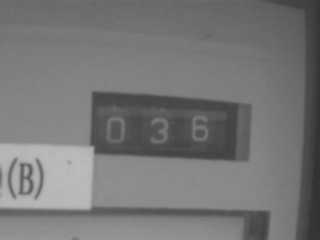
\includegraphics{gaussian.eps}
  \caption{$3\times 3$近似高斯模板}
  \label{fig:gaussian}
\end{figure}

直接计算模板较大的高斯滤波非常耗时。为了减少计算时间。由式\eqref{eq:gauss1}和式\eqref{eq:gauss2}可得。
\begin{equation}
  \label{eq:sep}
  g(x,y)=g(x)g(y)
\end{equation}
式\eqref{eq:sep}说明二维高斯函数可以用两个一维高斯函数的乘积表示,故$x$和$y$方向的高斯滤波互不影响。利用这一点,可以将二维的高斯滤波器分解为两个一维的高斯滤波器,分别在$x$和$y$方向进行滤波,从而减少运算量。

% \begin{enumerate}[(1)]
% \item 离模板中心越远的点,其权值逐渐减小到零。
% \item 总权值集中在$2\sigma$的范围内,故用标准差$\sigma$决定邻域的范围。
% \item 多个高斯滤波可以合并为一个高斯滤波过程。
% \item 对抑制高斯白噪声非常有效。
% \end{enumerate}

加权均值模板滤波的缺基本缺陷是抑制噪声和保留边缘的矛盾。模板越大,抑制噪声的效果越好,边缘也越模糊。这是因为当模板处在两块区域的边缘时,由于两块区域的灰度差别很大,取加权平均值导致边缘处的灰度差别变小,不利于后续的边缘检测。即用模板中心权值较大的高斯滤波模板,边缘也有一定的失真。为了做到既能减少噪声,又能保持边缘,可以采用中值滤波。中值滤波就是用模板下所有像素灰度的中值代替原像素值。由于只需知道第$\frac{1}{2}(n-1)$大的像素值,不需要知道其他像素值的相对大小,可以巧妙地改造快速排序算法求出快速地求出中值。选取数组中的某个值,如果将分割点和$\frac{1}{2}(n-1)$比较,发现当分割点小于$\frac{1}{2}(n-1)$,说明中值包含在较大的数组中,当分割点大于$\frac{1}{2}(n-1)$时,说明中值包含在较小的数组中。这时只需对包含中值的数组递归地采用上述分割方法。

\section{边缘检测}\label{sec:edge}

边缘是分割图像的一个重要特征。在灰度图像中,边缘表现为灰度有突然变化的区域。因此,边缘检测的经典算法是用每个像素所在邻域内的灰度变化确定边缘,而邻域内的灰度变化可以用邻域的导数刻画。这种利用利用邻域内的导数检测边缘,称为边缘检测局部算子法。

\subsection{一维信号边缘检测}

首先讨论一维信号的边缘检测算子,这不仅直观,也很容易推广到二维图像的边缘检测算子。而且一维信号的边缘检测算子也有实际用途,如用一维信号的边缘检测算子找出灰度直方图的波峰波谷。一维信号$f(x)$在邻域内的变化率用导数刻画:
\begin{equation}
  \label{eq:diff}
  \frac{\mathrm{d}f}{\mathrm{d}x}=\lim_{\Delta x\to 0}\frac{f(x+\Delta x)-f(x)}{\Delta x}
\end{equation}
连续信号$f(x)$无法直接观测,只能观测到间隔为1的离散信号$f(i)$,所以用差分$f'(i)=f(i+1)-f(i)$估计$f'(x)$。一阶差分相当于将模板$M'=[-1,1]$应用到一维信号中。模板$M'$的中心为左边的点。同理可得,$f(x)$的二阶导数可以用$f(i)$的二阶差分近似,相当于对$f(i)$应用模板$M''=[1,-2,1]$进行运算。

上述模板运算只利用了$i$和$i+1$处的值,和$i-1$没有关系。为了对称地利用$i$处的邻域,采用导数的对称的定义。
\begin{equation}
  \label{eq:diff2}
  \frac{\mathrm{d}f}{\mathrm{d}x}=\lim_{\Delta x\to 0}\frac{f(x+\Delta x)-f(x-\Delta x)}{2\Delta x}
\end{equation}
同样取$\Delta x=1$,得到一阶导数的近似值对应的模板为$M'_2=\frac{1}{2}[-1,0,1]$,二阶导数的近似值对应的模板为$M'_2=\frac{1}{2}[-1,-1,1,1]$。按照边缘处的一阶和二阶导数值分类,边缘可以分为阶跃形边缘、屋脊状边缘和斜坡形边缘。在阶跃形边缘处,一阶导数在此处存在一个脉冲,二阶导数在此处存在一个过零点。在屋脊状边缘处,一阶导数在此处存在阶跃,二阶导数在此处存在一个脉冲。在斜坡行边缘处,一阶导数在此处存在极值。如果发现导数存在这些特征,说明检测到边缘。

\subsection{二维图像边缘检测算子}

与一维图像的导数不同,二维图像的导数不仅有幅度,还有方向。图像$f(x,y)$可能在任意方向均存在导数。其中两个特殊的方向导数分别为沿着$x$和$y$轴方向的两个导数$f_x$和$f_y$,其他方向的导数都可以表示为这两个方向导数的线性组合。如果将$y$视为参量,则$f_x$可以视为以$x$为变量的一元函数,可以将模板$M'_2=[-1,0,1]$应用于$f(x,y)$求出该导数的近似值。然而,由于图像含有噪声,而且边缘不一定沿$x$方向,因此应该将模板应用于像素本身及其上下两个相邻像素,求出三个近似值,再求出这三个近似值的平均值作为该处$f_x$的估计值。这个计算过程相当于将如图\ref{fig:prewitt_x}所示的模板应用于图像$f(x,y)$。同理可得计算$f_y$的模板,如图\ref{fig:prewitt_y}所示。
\begin{figure}[!h]
  \centering
  \subfloat[x方向]{\label{fig:prewitt_x}\includegraphics{prewitt_x.eps}}\hspace{1cm}
  \subfloat[y方向]{\label{fig:prewitt_y}\includegraphics{prewitt_y.eps}}
  \caption{Prewitt算子}
\end{figure}
一种类似的算子是Sobel算子,如图\ref{fig:sobel}所示,它对中间一行运算的权值是上下两行的权值的两倍。
\begin{figure}[!h]
  \centering
  \subfloat[x方向]{\includegraphics{sobel_x.eps}}\hspace{1cm}
  \subfloat[y方向]{\includegraphics{sobel_y.eps}}
  \caption{Sobel算子}
  \label{fig:sobel}
\end{figure}

根据二元函数微分学,二维图像$f(x,y)$沿\emph{梯度}方向灰度变化最大。图像的梯度定义为向量$\nabla f=(f_x,f_y)$,梯度的幅值为$|\nabla f|=\sqrt{f_x^2+f_y^2}$,方向为$0=\arctan\left(\frac{f_y}{f_x}\right)$。为了减少计算量,梯度幅值一般简化为计算$\frac{1}{2}(f_x^2+f_y^2)$或$\max(|f_x|,|f_y|)$或$|f_x|+|f_y|$。另一种简化计算梯度的方法是利用与标准行列方向偏离45度的两个交叉的差分作为方向导数。这两个方向导数在$(i,j)$处的估计值为$f(i+1,j+1)-f(i,j)$和$f(i,j+1)-f(i,j+1)$。这两个差分运算可以用图\ref{fig:robert}所示的模板表示,称为Roberts算子。用上述算子求出梯度和幅值后,追踪具有高幅值的点,或追踪幅度极值点,可以得到边缘。
\begin{figure}[!h]
  \centering
  \subfloat{\includegraphics{robert_x.eps}}\hspace{1cm}
  \subfloat{\includegraphics{robert_y.eps}}
  \caption{Robert算子}
  \label{fig:robert}
\end{figure}

上述边缘算子的基本缺陷就是检测精度和抗噪声能力不能兼顾。由于图像的边缘和噪声均为灰度急剧变化的部分,简单的梯度运算会将噪声误认为边缘。Canny应用严格的数学方法分析边缘检测的缺陷,并提出平衡检测精度和抗噪声能力的方法。Canny给出了评价边缘检测的三个准则:
\begin{asparaenum}[(1)]
\item 信噪比准则:信噪比越大,边缘质量越高。
\item  定位精度准则,即检测出的边缘点尽量靠近实际边缘。
\item 单边缘响应准则:即单个边缘只产生一个响应,虚假边缘响应得到最大抑制。
\end{asparaenum}

为满足上述准则,Canny利用最优化方法,得到了最佳边缘模板。Canny针对一维边缘,推导出的最优边缘检测算子与高斯函数的导数类似。在实际应用中,为了减少计算量,可以用高斯滤波后再用Sobel算子求出方向导数的幅度和方向,用于近似计算Canny的最优边缘检测算子。

此时得到原始图像的梯度图像。梯度较大处都是边缘的候选点。但一个真实的边缘点附近往往有许多虚假的边缘响应,在图像中表现为一条较粗的边缘。为了细化边缘,在邻域内的多个边缘响应点只用保留一个。通过判断候选点是否为其梯度方向上的邻域的极大值判定该点是否为边缘点。具体做法是,对某个候选点,在其梯度方向上找出一个邻点,要求该邻点和候选点的连线与梯度方向相差不到45度。然后再其梯度的反方向上满足同样要求的邻点。比较候选点和这两个邻点的梯度幅值,如果候选点的梯度幅值高于两个邻点,则保留该候选点,否则删除该候选点。这一过程称为\emph{非极大值抑制}。
% \begin{algorithm}[H]
%   \caption{非极大值抑制}
% \label{alg:nms}
% \begin{algorithmic}
%   \REQUIRE $\textrm{梯度幅值图像}M\textrm{和梯度方向图像}D$
% \ENSURE $\textrm{边缘细化的梯度图像}N$
% \FOR {$i\gets 0$ \TO $\max(i)$}
% \FOR {$j\gets 0$ \TO $\max(j)$}
% \STATE $N_1[4]\gets\{(1,0),(1,1),(0,1),(-1,1)\}$
% \STATE $N_2[4]\gets\{(-1,0),(-1,-1),(0,-1),(1,-1)\}$
% \STATE $d\gets D(i,j) \mod \frac{\pi}{4}$
% \STATE $(u_1,v_1)\gets (i,j)+N_1[d]$
% \STATE $(u_2,v_2)\gets (i,j)+N_2[d]$
% \IF {$M(i,j) > M(u_1,v_1)$ \AND $(M(i,j) > M(u_2,v_2)$}
% \STATE $N(i,j)\gets M(i,j)$
% \ELSE
% \STATE $N(i,j)\gets 0$
% \ENDIF
% \ENDFOR
% \ENDFOR
% \end{algorithmic}
% \end{algorithm}

过极大值抑制后,边缘仅为单像素宽。然而这些边缘仍然存在虚假边缘响应点。使用双阈值的方法提高边缘质量。选取高低两个阈值。在梯度图像中找出幅度高出高阈值的点。,然后将这些邻点作为新的起点,再找出它们周围高于低阈值的邻点。

\section{图像分割}

图像分割就是将图像划分成多个区域,这些区域内的特征表现相似,而不同区域间特征显著不同。常见的特征有灰度、色彩、纹理和几何形状。图像分割的有两个目的。第一个目的是分离目标和背景,为图像识别奠定基础。第二个目的将像素组织成更高级的单元,进而从区域的角度而不是像素的角度更好地分析图像。
目前没有一种通用的分割方法,适用于各个领域,需要根据具体情况选择合适的分割算法。

\subsection{阈值分割}

阈值分割假定不同的区域的灰度值有显著差异,区域内的像素值在一个较小范围内浮动。许多图像满足这一假设。根据这一假设,找出各个区域的灰度区间,找出区间内的像素,即可完成分割。不同灰度区间的分界点称为\emph{阈值}。有多种方法可以选取阈值。最简单的情况是选取单阈值,将图像分割为低于阈值的部分和高于阈值的部分。还有双阈值的情况,即选取一个较高的阈值和较低的阈值,将图像分割为处于高低阈值之间的区域,和在高低阈值之外的区域。阈值可以由用户指定,但为了自动处理和识别图像,应根据图像的特点计算合适的阈值。

计算阈值的基本依据是直方图。如果能估计待分割区域的占整个图像的百分比$p$,则找出一个阈值,使低于(高于)阈值部分的灰度出现概率为$p$即可完成分割。如果区域的百分比不能确定,可以根据直方图的波峰和波谷计算阈值。直方图的波峰对应区域内像素的平均灰度,波谷对应区域边界的灰度,因此选取两个波峰之间的波谷对应的灰度作为阈值。如果两个区域的灰度有重叠,直方图的波峰波谷不明显,或区域之间的面积比例悬殊,该方法的分割效果不理想。

自动确定阈值的另一种常见方法是Otsu算法。该算法假定目标和背景区域分别为黑白两种像素,或图像的直方图呈现双模式分布。设$P(i)$表示灰度$i$出现的概率,$t$为候选阈值,$\mu_1(t)$和$\sigma_1^2)$分别表示低于阈值$t$的区域的均值和方差,$\mu_2(t)$和$\sigma_2^2(t)$分别表示高于阈值$t$的区域的均值和方差,$q_1(t)$和$q_2(t)$分别是两个区域的灰度百分比。则组内方差$\sigma_W^2(t)$的定义为:
\begin{equation}
  \label{eq:sigw}
  \sigma_2^2(t)=q_1(t)\sigma_1^2(t)+q_2(t)\sigma_2^2(t)
\end{equation}

其中
\begin{equation}
  \label{eq:musig}
  \begin{aligned}
    q_1(t) &= \sum_{i=0}^tP(i) \quad & q_2(t) &= \sum_{i=t+1}^{L-1}P(i) \\
    \mu_1(t) &= \sum_{i=0}^t\frac{iP(i)}{q_1(t)} \quad & \mu_2(t) &= \sum_{i=t+1}^{L-1}\frac{iP(i)}{q_2(t)} \\
    \sigma_1(t) &= \sum_{i=1}^t\frac{[i-\mu_1(t)]^2}{q_1(t)} \quad & \sigma_2(t) &= \sum_{i=t+1}^{L-1}\frac{[i-\mu_2(t)]^2}{q_2(t)}
  \end{aligned}
\end{equation}

Otsu算法找出使组内方差最小$\sigma_W^2(t)$的$t$作为阈值。如果直接按式\ref{eq:sigw}计算所有可能的$t$值,则对每个$t$值都需要分别求出两个区域的均值和方差,计算效率低下。可以用总方差和组内方差的关系简化计算。总方差的定义为:
\begin{equation}
  \label{eq:var}
  \sigma^2=\sum_{i=1}^{L-1}(i-\mu)^2P(i)
\end{equation}
由\eqref{eq:sigw}和\eqref{eq:var}可得:
\begin{equation}\begin{split}
  \label{eq:sigrel}
  \sigma^2 =&[q_1(t)\sigma_1^2(t)+q_2(t)\sigma_2^2(t)] \\
  &  +\{q_1(t)[\mu_1(t)-\mu]^2+q_2(t)[\mu_2(t)-\mu]^2\}
\end{split}\end{equation}
式\eqref{eq:sigrel}的第一项是组内方差$\sigma_W^2$,第二项是组间方差$\sigma_B^2$。由于总体方差和$t$无关,故组内方差最小时,最间方差最大,故通过计算每个$t$值的组内方差找出阈值。总均值$\mu$和两个区域的均值$\mu_1(t),\mu_2(t)$和百分比$q_1(t),q_2(t)$的关系为:
\begin{equation}
  \label{eq:sigma}
  \mu=q_1(t)\mu_2(t)+q_2(t)\mu_2(t)
\end{equation}
将式\eqref{eq:sigma}代入式\eqref{eq:sigrel},消去$\mu$,组间方差可以简化为:
\begin{equation}
  \label{eq:sigb}
  \sigma_B^2(t)=q_1(t)q_2(t)[\mu_1(t)-\mu_2(t)]^2
\end{equation}
找出使$\sigma_B^2(t)$最大的$t$值,作为Otsu算法的阈值,用公式表示为:
\begin{equation}
  \label{eq:otsu}
  t^{*}=\arg\max_{0\leqslant t\leqslant L-1}\sigma_B^2(t)
\end{equation}

如果图像的背景亮度不均匀,则全局阈值分割效果不理想,因为不同的区域平均亮度有差别,对平均亮度不同的区域使用相同的阈值,导致部分像素被错分。这种情况可以使用局部阈值法。局部阈值法对每个像素的邻域均计算一个局部阈值,比较局部阈值和像素灰度确定像素所在的区域。局部阈值法的缺点是计算量比全局阈值法大,容易在目标区域内形成裂痕或空洞,而且邻域的大小严重影响分割效果。因此应根据图像的特点选择邻域大小和局部阈值的计算方式。


% 式\eqref{eq:sigb}的四项$q_t(t),q_2(t),\mu_1(t),\mu_2(t)$可以用递推公式计算,计算方式为:
% \begin{subequations}
%   \begin{align}
%     q_1(t+1) &= q_1(t)+P(t+1) \\
%     q_2(t+1) &= 1-q_1(t) \\
%     \mu_1(t+1) &= \frac{q_1(t)\mu_1(t)+(t+1)P(t+1)}{q_1(t+1)} \\
%     \mu_2(t+1) &= \frac{\mu-q_1(t+1)\mu_1(t+1)}{1-q_1(t+1)}
%   \end{align}
% \end{subequations}

\subsection{边缘分割}

边缘分割利用图像的边缘分割图像。用\ref{sec:edge}节所述的边缘检测算子找出边缘点后,再将边缘点连成轮廓线,分割轮廓线两边的区域。边缘检测算子容易产生虚假的边缘又丢失部分边缘,从而产生边缘缺口。如果轮廓线的曲线类型已知,如直线或圆等,则用哈夫变换对于有缺口的边缘也能产生较好的分界线。哈夫变换的基本思想就是借助带参曲线方程,先将图像空间的点变换成参数空间的曲线集合,再将参数空间的曲线交点变换成图像空间的曲线集合。下面以边缘直线检测为例介绍哈夫变换。

首先要定义带参直线方程。直线方程通常的定义为:
\begin{equation}
\label{eq:scope}
  y=kx+b
\end{equation}
式\eqref{eq:scope}不能表示和$x$轴平行的直线,这是由于参数$k$只能取有限值。更好的参数向量是原点到直线的垂直向量,用向量的长度$\rho$和倾斜角$\theta$表示。带参数$\rho$和$\theta$的直线方程为:
\begin{equation}
  \label{eq:polar}
  \rho=x\cos\theta+y\sin\theta
\end{equation}
式\eqref{eq:polar}可以表示任意方向的直线,因此作为带参直线方程。对于给定的$(x,y)$,参数方程可以看作参数空间的一条正弦曲线。由于正弦函数具有周期性,$\theta$只用取$[0,2\pi)$范围内的值。设图像中有$n$个点$(x_1,y_1),(x_2,y_2),\cdots,(x_n,y_n)$。这些点的方程分别为:
\begin{equation}
\label{eq:func}
  \rho=x_i\cos\theta+y_i\sin\theta,\quad i=1,2,\cdots,n
\end{equation}
式\eqref{eq:func}说明这$n$个点对应参数空间的$n$条正弦曲线。若这些点共线,则存在一条参数为$\rho_0$和$\theta_0$的直线$\rho_0=x\cos\theta_0+y\sin\theta_0$。将$(x_i,y_i)$代入直线方程,不难看出$(\rho,\theta)$为式\eqref{eq:func}表示的一组曲线的交点。故在参数空间中找出交点,即可找出图像的直线。

从曲线的方程求出交点非常困难,所以我们将曲线“画”出曲线的图像。而要画出曲线图像,需要对参数空间进行离散化。分别指定$\rho$和$\theta$的很小的量化间隔$\Delta\rho$和$\Delta\theta$,得到$\rho$和$\theta$的一组离散值。对每对离散的$(\rho,\theta)$指定一个像素值$A(\rho,\theta)$。这些像素构成一个二维的\emph{累加器数组},其初值均为零。对$\theta$的所有离散值$\theta'$,计算对应的$\rho$值。然后量化$\rho$,即找出最接近$\rho$的离散值$\rho'$。然后将累加器数组内位于$(\theta',\rho')$处的值加1,表示曲线通过该像素。显然,累加器数组的值表示通过该处的曲线数,对应于边缘图像共线的点数。累加器数组的峰值是曲线的多重交点,对应边缘图像中共点最多的直线,即为检测出的直线。

\section{二值图像分析}

图像分割后的结果一般是二值图像,其中目标像素值设为1。背景像素值设为0。在文档扫描和工业机器视觉系统中,计算机系统都是以二值图像作为识别的对象。二值图像算法的应用场合十分广泛,例如目标计数、定位和识别等。

\subsection{连通成分标记}\label{sec:comp}

\emph{连通成分}指具有相同的灰度且其中任意像素都有相邻像素的像素集合。连通成分标记就是用不同的标号区分不同的连通成分,每个连通成分的像素值设定为其所在的连通成分的标号。标记连通成分有两种基本算法:\emph{递归搜索算法}和\emph{逐行扫描算法}。

递归搜索算法的基本思想是将某个具有最大灰度的像素作为种子像素,将其像素值设定为连通成分的标号。再从其相邻的像素中找出未标记且值为1的像素,将这些像素作为新的种子像素,递归地施行上述方法,直到标记完连通成分的所有像素。然后找出另一连通成分的种子像素,施行同样的方法,直至标记出所有的连通成分。%设$B$表示二值图像,$LB$表示连通成分的标记图像,$LB(i,j)$的初值为0,则算法如\ref{alg:comp}所示。
% \begin{algorithm}[H]
%   \caption{标记二值图像的连通成分}
%   \label{alg:comp}
%   \begin{algorithmic}
%     \REQUIRE $\textrm{二值图像}B$
%     \ENSURE $\textrm{连通成分标记}LB$
%     \STATE $label\gets 0$
%     \FOR{$i\gets 0$ \TO $M-1$}
%     \FOR{$j\gets 0$ \TO $N-1$}
%     \IF{$B(i,j)=1$ \AND $LB(i,j)=0$}
%     \STATE $label\gets label+1$
%     \STATE $\search(i,j,label)$
%     \ENDIF
%     \ENDFOR
%     \ENDFOR
%     \STATE $\textbf{procedure}\ \search(i,j,label)$
%     \STATE $LB(i,j)\gets label$
%     \STATE $N\gets \neighbours(i,j)$
%     \FOR{$(i',j')\in N$}
%     \IF{$B(i',j')=1$ \AND $LB(i',j')=0$}
%     \STATE $\search(i',j',label)$
%     \ENDIF
%     \ENDFOR
%   \end{algorithmic}
% \end{algorithm}

在递归扫描算法中,每扫描一个像素就要做一次递归。数字图像的像素点很多,递归深度非常大,因此算法的时间和空间开销非常大。有人提出了逐行扫描算法,只需扫描图像两次。该算法扫描图像时,找出未标记的像素作为种子像素,设定其临时标号,将种子像素的临时标号传播到后续像素。由于种子像素的标号只能向右下转播,故其左下方也可能存在另一个种子像素\footnote{种子像素$P$的右上方也有可能存在种子像素$Q$。在这种情况下,我们将像素$Q$当作“当前”像素,则$P$仍然是“左下方”的像素。左上方的种子像素和“当前”种子像素不可能在同一个连通成分内,否则左上方的种子像素会将标号传播到“当前”种子像素,此时“当前”像素不是种子像素。所以只用考虑合并“当前”像素及其左下方像素的传播区域。}两个种子像素的标号可能传播到同一区域。如果出现这种情况,说明两个种子像素传播的区域在同一个连通成分内,说明这两个临时标号其实标记了同一个连通成分,是两个等价的标号。为了确保同一连通成分内只有一个标号,需要再次扫描图像,将临时标号用其等价标号代替。

\subsection{数学形态学}

\emph{数学形态学}是建立在集合代数理论上,分析几何形状和结构的数学的学科,最初用于岩石结构分析。形态学的主要用途是获取并改变物体的拓扑结构。通过将结构元作用于几何形状,可以得到物体更本质的形态。进入八十年代,数学形态学被引入机器视觉领域后,人们对其进行深入的研究和广泛的应用。至今理论上已趋于完备,应用领域上不断拓展,应用到平滑滤波、边缘检测、特征提取、形状描述、模型构造等图像处理的方方面面。

\emph{二值形态学}是数学形态学最简单的情况,它具有运算简单、效果显著的特点。二值形态学运算是用一个较小的二值图像在图像上进行运算。这个较小的图像称为\emph{结构元}。在定义形态学运算前,先定义\emph{平移}运算。设$A$表示几何形状的像素坐标集合,则有序对$b$对$A$平移运算定义为对$A$的每个坐标加上有序对$b$,用公式表示为:
\begin{equation}
  \label{eq:shift}
  A_b=\{a+b|a\in A\}
\end{equation}

二值形态学最基本的运算是\emph{膨胀}和\emph{腐蚀}。设二值图像值为1的像素的坐标集合为$A$,结构元中值为1的像素坐标集合为$B$,则定义$A$关于$B$的膨胀运算为用$B$内所有坐标对$A$进行平移,记为$A\oplus B$,如下所示:
\begin{equation}
  \label{eq:dilate}
  A\oplus B=\bigcup_{b\in B}A_b=\{a+b|a\in A,b\in B\}
\end{equation}

式\eqref{eq:dilate}是从集合的角度定义膨胀运算,也可以从图像的角度直观地定义膨胀运算。从图像上看,膨胀运算相当于结构元在图像上移动,让结构元中心与像素重合,当遇到值为1的像素时,将结构元上的值和结构元下对应位置的像素做“或”运算。图\ref{fig:binary}和图\ref{fig:struct}分别是二值图像和结构元,图\ref{fig:dilate}是两者的膨胀运算结果。从图上看出,膨胀运算使形状的区域扩大。
\begin{figure}
  \centering
  \subfloat[二值图像]{\label{fig:binary}\includegraphics{binary.eps}}\hspace{1cm}
    \subfloat[结构元]{\label{fig:struct}\includegraphics{struct.eps}}
  \caption{二值图像和结构元}
\end{figure}

定义$A$关于$B$的腐蚀运算为,用$B$中所有坐标对$A$进行平移运算后,找出仍然在$A$中的坐标,将这些坐标组成一个集合。腐蚀运算记为$A\ominus B$,用公式表示为:
\begin{equation}
  \label{eq:erode}
  A\ominus B=\{a|(a+b)\in A\quad\textrm{for}\ a\in A,b\in B\}=\bigcap_{b\in B}A_b
\end{equation}

从图像上看,腐蚀运算也是将结构元中心在图像上移动,只有当结构元上值为1的位置覆盖的像素值均为时,才将结构元和其覆盖的像素进行“或”运算。腐蚀运算的结果如图\ref{fig:erode}所示。从图上发现,腐蚀运算使区域缩小。
\begin{figure}
  \centering
  \subfloat[膨胀运算]{\label{fig:dilate}\includegraphics{dilate.eps}}\hspace{1cm}
    \subfloat[腐蚀运算]{\label{fig:erode}\includegraphics{erode.eps}}
  \caption{膨胀和腐蚀运算}
\end{figure}

在腐蚀和膨胀运算的基础上定义开运算和闭运算。开运算就是腐蚀再膨胀,记为$A\circ B=(A\ominus B)\oplus B$。闭运算就是膨胀再腐蚀。图\ref{fig:open}和图\ref{fig:close}分别是开运算和闭运算的结果。
\begin{figure}
  \centering
  \subfloat[开运算]{\label{fig:open}\includegraphics{open.eps}}\hspace{1cm}
  \subfloat[闭运算]{\label{fig:close}\includegraphics{close.eps}}
  \caption{开运算和闭运算}
\end{figure}


%%% Local Variables: 
%%% mode: latex
%%% TeX-master: "thesis"
%%% End: 


\chapter{机器视觉库OpenCV}

\section{概述}

本文的算法实现基于OpenCV,OpenCV降低了开发图像识别程序的难度,提高了计算效率。OpenCV的全称是open source computer vision library,是一个开源的计算机视觉库,用于图像处理、机器视觉、模式识别、机器学习、计算机建模和虚拟现实等领域。OpenCV由英特尔公司发起,旨在为CPU计算密集型任务提供软件支持\upcite{opencvref}。OpenCV具有如下特性:
\begin{asparaenum}[(1)]
\item 提供大量的算法。OpenCV提供人机交互、图像分割、运动追踪、三维建模、特征识别、目标识别、图像匹配、机器学习等领域的大量算法,涵盖图像处理、机器视觉和模式识别的方方面面。
\item 用C/C++开发。在早期的OpenCV版本中,绝大部分程序由C语言开发。最新的版本主要用C++语言开发。与用C语言开发的早期版本相比相比,用C++开发的新版本在兼容性、类型安全、类型推断、自动内存管理和并行计算优化等方面有显著优势。
\item   为多种程序设计语言提供接口。OpenCV原生接口是是C++语言。为了与早期版本兼容,也提供了C语言接口。为了便于Python和Java程序员开发机器视觉应用,OpenCV也提供了Python和Java语言的接口\upcite{opencvtut}。
\item 支持多种平台。OpenCV支持Windows,Linux,Mac OS,iOS和Android平台。
\item 效率高,实时性强。OpenCV专注于计算效率和实时性,因此OpenCV提供的算法实现具有较快的速度。同时OpenCV针对多核CPU、CUDA和OpenCL等并行计算平台进行优化,进一步加快了OpenCV的计算速度\upcite{opencvtut}。
\end{asparaenum}

\section{基本数据结构}

\subsection{向量数据结构}

在图像处理和机器视觉中,OpenCV用几种向量数据结构表示点、矩阵的行列、颜色值、特征向量等。表示点的数据结构有二维坐标类Point\_和三维坐标类Point\_\upcite{opencvref}。这两个类都支持坐标的加减运算$P_1\pm P_2$,坐标的缩放运算$kP$等。Vec类是通用的向量类,它表示任意长度、任意类型元素的向量。Scalar类是Vec类的特例,表示包含分量不多于四个的双精度浮点数向量\upcite{opencvref}。在OpenCV的库函数中,Scalar类一般用于指定颜色值,如在绘制线段的函数lines中,如果指定Scalar类为$(100,100,100)$,则线段颜色的RGB值均为100。

\subsection{矩阵数据结构}


图像处理和识别需要进行大量的矩阵运算。OpenCV用Mat类表示矩阵。Mat类能表示任意大小、任意维度的矩阵,矩阵的元素可以为字节、整数、浮点数。Mat类也可以表示多通道的矩阵,其每个元素为向量,用于记录该处所有通道的值\upcite{opencvref}。一维矩阵的Mat类可以和点、向量、数字等数据结构进行相互转化。由于Mat类表示的矩阵类型多种多样,一维向量、二维矩阵、灰度图像、彩色图像、点云、张量、直方图等数据均可用Mat类存储\upcite{cookbook}。

Mat类使用引用计数进行自动内存管理,使用户不必手动进行内存管理,提高了内存管理效率,避免了内存泄露和无效指针等内存管理错误\upcite{opencvtut}。创建矩阵时,Mat类为矩阵数据分配内存,然后将引用计数置为1。矩阵占用大量内存,为了减少内存使用量,Mat类对象进行赋值运算$A=B$时,仅仅将$B$维数、大小等信息复制到$A$中,让$B$和$A$共享矩阵数据,然后将相应的引用计数加1。销毁Mat类对象时,先将其矩阵数据的引用计数减1,只有引用计数为0,即没有Mat类对象指向这块数据时,才释放数据\upcite{opencvref}。

Mat类支持许多矩阵运算,如矩阵加减$A\pm B$,矩阵与标量的乘法$kA$,矩阵与矩阵的乘法$A\times B$,转置$A^T$。如果两个Mat类对象都表示向量,还能计算向量的点积$A\cdot B$和叉积$A\times B$。除上述双目运算外,Mat类还支持几个单目运算,如矩阵的模、矩阵元素总和及均值、矩阵的迹和行列式等\upcite{opencvref}。

由于Mat类表示的矩阵多种多样,其构造函数也有多个\upcite{opencvref}。最简单的是Mat(),表示创建一个$3\time 3$矩阵。这个简单的构造函数广泛地用于滤波和形态学运算。另一个常见的构造函数是Mat(int rows, int cols, int type),表示创建一个行数为rows,列数为cols,元素类型为type的二维矩阵。一维矩阵的Mat类可以用构造函数Mat(Vec \& vec)从向量vec转化而来。高维矩阵的Mat类可以用构造函数Mat(int ndims, int sizes[], int type)创建,其中ndims,sizes[]和type分别表示维数、每个维度的行数和元素类型。

除了Mat类外,还有其他几个类可以表示矩阵。例如表示小尺寸矩阵的Matx类。Matx类在编译时就确定矩阵的大小和元素类型,适用于表示滤波模板和形态学的结构元等大小和元素值确定的模板。Matx类支持Mat类的大部分运算。如果某种运算在Matx类中没有实现,可以将Matx类转换成Mat类再计算。另一个表示矩阵的类是SparseMat。它内部只存储所有非零元素,因此特别适合表示大型高维稀疏矩阵。

\section{相关模块}

OpenCV实现了图像处理、机器视觉和模式识别的许多常见算法。由于实现的算法繁多,OpenCV按领域分成多个模块。目前OpenCV包括核心、图像处理、图形界面、视频分析、三维相机定标、特征识别、目标识别、机器学习、GPU加速等模块。本文使用了OpenCV的图像处理、图形界面两个模块。

OpenCV的图像处理模块涉及许多常见的图像处理方法,如滤波、几何变换、颜色空间变换、二值化、边缘检测和直方图变换等\upcite{opencvref}。在滤波子模块,OpenCV除了提供常见的滤波器外,还支持用户自定义的滤波器。自定义的滤波器可以合并其他处理步骤,如颜色空间转换和二值化等,从而提高程序性能。OpenCV提供了多种二值化算法,支持多个颜色空间之间的转换,包含了多种边缘检测算子和直方图变换技术,便于开发图像处理程序。

在图形界面模块,OpenCV支持创建简单窗口并在窗口显示图像。为了便于在图像处理程序中调整参数,OpenCV提供了创建滑块的函数,通过移动滑块控制参数。OpenCV的图形界面函数非常简单,调用几个函数就可以创建有简单的交互功能的图像处理程序,使用户不必了解图形界面的细节,将精力集中到实现图像处理算法中。

%在机器学习模块,OpenCV实现了贝叶斯分类、k近邻算法、支持向量机、决策树和神经网络等多种机器学习算法。只需提供样本,OpenCV就能计算分类器的参数,对未知样本分类。

%%% Local Variables: 
%%% mode: latex
%%% TeX-master: "thesis"
%%% End: 



\chapter{算法实现}

\section{概述}

摄像头拍摄的是彩色图像,如图\ref{fig:src}所示。从图上看出,不同电流表的数字形状和大小相同,给识别带来了方便。然而,数字只占整幅图像很小的一部分。电流表在黑色边框中,而电流表指针和电流表右侧也有黑色边框。防护玻璃表面有反光、灰尘,数字的黑色边框亮度不均匀,图像中又含有噪声。这些都给数字识别带来了干扰。因此,在识别数字前,必须首先减少噪声,排除无关部分的干扰。为此,本文将读数识别分成预处理、数字边框定位、数字分割和数字识别四个过程。其中预处理用于增强图像质量,数字边框定位通过找出黑色边框找出数字的大致位置,数字分割则精确地分割出数字的像素,数字识别则用于识别分割的数字。

\begin{figure}[h]
  \centering
  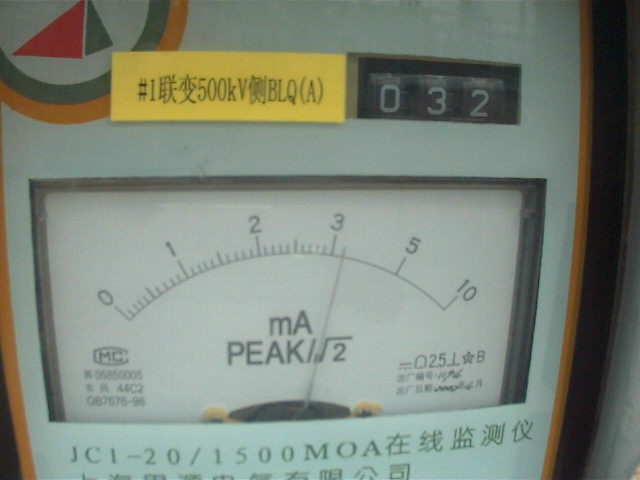
\includegraphics[scale=0.5]{src.png}
  \caption{原始图像}
  \label{fig:src}
\end{figure}

\section{图像预处理}

受光照条件和噪声等因素的影响,图像的质量不佳,不能直接用于数字识别\upcite{imgproc}。需要进行预处理,改善图像质量,从而更容易识别数字。本文采用的预处理方法先后有\emph{灰度化},\emph{高斯滤波}和\emph{直方图均衡}。

\subsection{灰度化}



由于待识别的数字在右上角,所以只需截取右上部分做后续处理,如图\ref{fig:rgb}所示。首先将彩色图像转换成灰度图像。这样做的原因是:
\begin{asparaenum}[(1)]
\item 灰度图像只有一个分量,比三分量的彩色图像更易处理;
\item 本文识别的数字边框为黑底白字,边框内绝大部分像素都是黑白颜色,灰度化后颜色基本没有变化。
\end{asparaenum}

本文使用OpenCV建议的加权平均法求出灰度图像,OpenCV给出的公式为$I=0.114R+0.587G+0.299B$。灰度图像如\ref{fig:gray}所示。

\begin{figure}[h]
  \centering
  \subfloat[彩色图像]{\label{fig:rgb}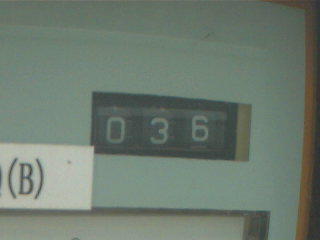
\includegraphics[scale=0.5]{rgb.png}}\hspace{1in}
  \subfloat[灰度图像]{\label{fig:gray}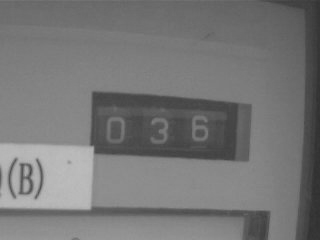
\includegraphics[scale=0.5]{gray.png}}
  \caption{灰度化}
\end{figure}

\subsection{高斯滤波}


灰度图像含有较多噪声,不利于提取目标,需要用图像平滑的方法减少噪声。观察发现,待处理图像的噪声以盐椒噪声为主,因此选用高斯滤波进行平滑滤波\upcite{imgproc}。在调用OpenCV的高斯滤波函数时,要指定高斯滤波模板的长宽,$\sigma$值和边界扩充类型。一般情况下,只需使用长宽相等的高斯滤波模板。模板尺寸越大,平滑的效果越好,但图像的边缘也越模糊。综合以上情况,将长和宽均设置为3。$\sigma$值的设定也有一定的要求。高斯函数在半径为$2\sigma$范围内的积分为0.95,故绝大部分权值集中在这个领域内。为了最大限度地发挥高斯滤波的效果,需要保证模板能覆盖这个邻域,故选择$\sigma=2/3$。边界扩充类型指将高斯滤波模板中心与图像边界重合,模板覆盖的部分像素超出图像边界时,这部分像素值的计算方式。一般的做法是将边界内的像素值复制到边界外。高斯滤波的效果如\ref{fig:gauss}所示。
\begin{figure}[h]
  \centering
  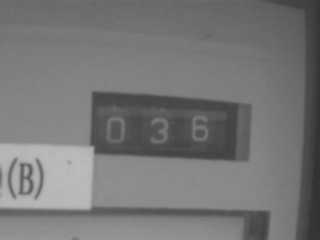
\includegraphics[scale=0.5]{gaussian.png}
  \caption{高斯滤波}
  \label{fig:gauss}
\end{figure}

\subsection{直方图均衡}


由于不同时间内光照条件不同,不同时间采集的图像的整体亮度不同。例如日光微弱时图像整体偏暗,日光强烈时图像整体偏亮。偏暗和偏亮的图像对比度不高,不利于识别。因此,采用直方图均衡化的方法增强图像的动态范围,从而达到增强图像整体对比度的效果。在进行直方图均衡化前,需要进行图像平滑。这是因为直方图均衡对图像的所有像素的灰度不加选择地加以扩充,因此噪声的灰度也被扩充,使原本灰度相近的区域灰度差距加大,对图像分割造成不利影响。因此本文把直方图均衡化放在高斯滤波后进行。

比较均衡化前的直方图\ref{fig:histsrc}和均衡化后的直方图\ref{fig:histequal}分别是均衡化前和均衡化后的直方图,可以发现均衡化后的直方图比均衡化前的直方图具有更宽的动态范围,每个灰度级上有大致相等的像素数。
\begin{figure}[h]
  \centering
  \subfloat[均衡化前的直方图]{\label{fig:histsrc}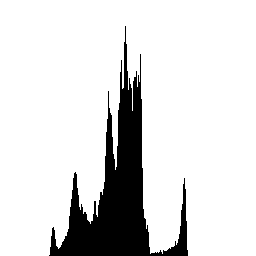
\includegraphics[scale=0.5]{histsrc.png}}
  \subfloat[均衡化后的直方图]{\label{fig:histequal}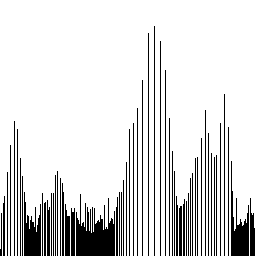
\includegraphics[scale=0.5]{histequal.png}}
  \caption{均衡化前后的直方图}
\end{figure}
直方图均衡化后的图像如图\ref{fig:equal}所示。经直方图均衡化后,不同时间的图像灰度分布大致相同,对于图像分割和识别是十分有益的。
\begin{figure}[h]
  \centering
  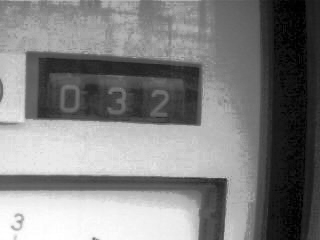
\includegraphics[scale=0.5]{equal.png}
  \caption{直方图均衡化}
  \label{fig:equal}
\end{figure}



\section{数字边框定位}

数字边框定位是电表读数识别的一个关键环节,也是较难的环节。数字边框内的数字是待识别的目标,数字边框外的图像则为无用信息。直接从原图中提取数字,难度大,准确率低。因此,应首先找出数字边框,去除无用的部分。观察图\ref{fig:equal}发现,数字边框周围有一些干扰区域,如右侧的电表边框和下侧的指针边框颜色灰度和数字边框的背景类似。这些干扰区域增加了分割的难度。

\subsection{二值化}

数字边框定位的第一步是二值化,即将原图分割为目标区域和背景区域,将目标区域的灰度设为255,背景区域的灰度设为0。观察图像发现,图像的各个区域内灰度差别较小,区域间灰度差别较大,适合用阈值法分割。阈值分割的关键是找到阈值。由于本文的灰度图像由大片的黑色和白色区域组成,可以使用Otsu算法分割阈值,

由式\eqref{eq:otsu}可得,Otsu算法需要对每个可能的灰度$t$计算$q_1(t),q_2(t),\mu_1(t),\mu_2(t)$四项。如果直接根据式\eqref{eq:musig}计算这四项,计算过程复杂而低效。为了简化计算,可以将式\eqref{eq:musig}改写成递推公式:
\begin{equation}
  \label{eq:recursive}
  \begin{aligned}
    q_t(t+1) &=q_1(t)+P(t+1)\\
    q_2(t+1) &=1-q_1(t) \\
    \mu_1(t+1) &=\frac{\mu_1(t)q_1(t)+(t+1)q_1(t+1)}{q_1(t+1)} \\
    \mu_2(t+1) &=\frac{\mu-q_1(t+1)\mu_1(t+1)}{q_2(t+1)}
  \end{aligned}
\end{equation}
递推公式\eqref{eq:recursive}含有总体均值$\mu$,需要在遍历$t$计算这四项之前计算。设定这四项的初值$q_1(0)=0,q_2(0)=1,\mu_1(t)=0,\mu_2(t)=\mu$,从$t=0$开始计算这四项,每增加一次$t$值,就更新这四项的值。如果小于某个$t$值的区间均值$q_1(t)$极小,则其方差$\mu_1(t)$极大,这个区间的像素极少,这样的$t$值必然不能作为分割点。同理,如果$t$值过大,导致大于$t$的区域的像素极少,同样不能作为阈值。因此计算$q_1(t)$和$q_2(t)$后,如果其中一项小于一个很小的门限,则这时的$t$值不能作为阈值,应直接进入下一轮循环。确保$t$值有效后,再用式\eqref{eq:sigb}更新组间方差$\sigma_B^2$,如果大于目前最大的$\sigma_B^2$值,则将阈值$t^{*}$更新为$t$。遍历$t$的所有取值后,即找出阈值$t^{*}$。分割结果是二值图像,如图\ref{fig:otsu}所示。从图上看出,数字也分割了出来,可以直接从图中找出数字。然而,这只是数字的初步分割。对于绝大多数电流表图像,这种初步分割得到的数字轮廓不准确,所以需要在数字边框定位后,在数字边框内的小块图像对数字进行精确定位。

\begin{figure}[h]
  \centering
  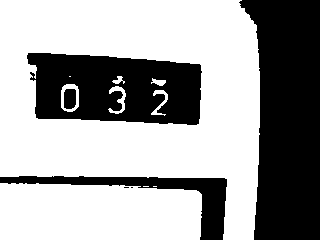
\includegraphics[scale=0.5]{otsu.png}
  \caption{Otsu算法}
  \label{fig:otsu}
\end{figure}


\subsection{连通成分筛选}

观察图\ref{fig:otsu}可得,二值化的图像黑色部分不仅包含数字边框,还包含其他几个区域,如电流表指针盘的边框和右侧的边框。这些区域需要去除,只保留数字边框。


由于这几个区域都是黑色区域,为了区分这几个区域,可以用连通成分标记算法给不同的区域赋予不同的标记。一般情况下,区域内可能有空洞或裂痕,连通成分标记可能失效。但这里的图像二值化的效果较好,区域内部不存在裂痕,适合用连通成分标记算法处理。本文选用\ref{sec:comp}节介绍的逐行扫描算法进行连通成分标记。逐行扫描算法使用并查集记录等价关系。扫描过程中算法对并查集进行大量的$\union$和$\find$操作,因此$\union$和$\find$操作的效率关系到算法的效率。

为优化$\find$和$\union$操作,可以使用如下两种策略。第一种策略是\emph{按秩合并}\upcite{alg},对任意元素$x$,它的\emph{秩}定义为从该结点到其后代结点的最长路径的边数的上界,记作$rank[x]$。当用$\make(x)$创建仅包含元素$x$的集合时,$rand[x]=0$。所有$\find(x)$操作不改变$rank[x]$。进行$\union(x,y)$操作时,比较结点$x$和结点$y$的祖先的秩,如果不相等,将秩较低的根结点指向秩较高的根结点,两者的秩不增加;如果相等,则任选一个根结点指向另一个根结点,并增加新的根结点的秩。另一种策略是\emph{路径压缩}\upcite{alg}。它用于$\find(x)$操作,将其访问的所有的结点都直接指向根结点。连通成分标记算法的结果如图\ref{fig:candidate}所示,不同区域已经用不同的灰度区分。

%用并查集使逐行扫描算法更加高效。算法第一次扫描,找到种子像素时,设定一个标号,并在并查集中创建一个只包含该标号的集合。在将标号传播到右下方的邻接点的过程中,如果发现两个不同的标号传播到同一个像素,只传播较小的标号,并将两个标号所在的集合合并。第一次扫描结束后,所有标号所在的集合均已确定。在第二次扫描时,将像素的标号改成该标号所在集合的代表标号。


\begin{figure}[h]
  \centering
  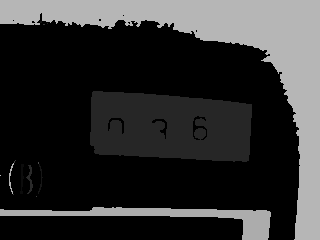
\includegraphics[scale=0.5]{candidate.png}
  \caption{连通成分}
  \label{fig:candidate}
\end{figure}


标记完各个连通成分后,下一步是从中找出数字边框。对这些连通成分进行分析。首先对连通成分进行初步分析,得到每个连通成分的基本特征,如像素数$n$和包围连通成分的最小矩形的长$L$和宽$W$等。在这些基本特征的基础上可以得到另一些特征。如长宽比$r=L/W$,面积$S=L\times R$等。再定义连通成分的区域密度为$\rho=n/S$。通过人工找出多幅图像内数字边框,综合它们的连通成分的基本特征的范围,得到数字边框对应的连通成分的各个特征具有如下范围:
\begin{equation}
  \label{eq:range}
  \begin{cases}
    8000  <  p  <  10000 \\
1.9  <  r  <  2.9 \\
0.6  <  \rho  < 0.9 
  \end{cases}
\end{equation}
因此,对每个连通成分计算这些特征值,发现落在式\eqref{eq:range}所示范围的,可以认定为数字边框。找出的数字边框如图\ref{eq:frame}所示。
\begin{figure}[h]
  \centering
  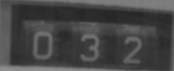
\includegraphics[scale=0.5]{frame.png}
  \caption{数字边框}
  \label{eq:frame}
\end{figure}

\subsection{倾斜校正}

因拍摄的角度问题,数字及其边框有一定的倾斜角度。因此找出数字边框后,为便于数字分割与识别,应对数字边框图像进行倾斜矫正。具体做法是先找出数字边框的上下两条横线,这两条横线的倾斜角度作为整个数字边框的倾斜角度,然后根据倾斜度旋转图像,使边框水平。

用边缘检测算子可以找出上下两条横线。由于数字边框较小,虚假的边缘对横线的倾斜角度有较大影响,边缘检测应尽量准确。为了提高边缘检测的准确度,减少虚假边缘,本文使用Canny边缘检测算子。OpenCV实现了边缘检测算子函数,但需要提供高低两个阈值和梯度的计算方式。由\ref{sec:edge}节可知,高低阈值用于Canny算子的非最大值抑制过程,只有高于这两个阈值的边缘才得以保留。这两个阈值可以在进行仪表自动识别前确定。具体做法是用Sobel算子或Prewitt算子求出原始图像的梯度图像,由于需要保留的边缘数字边框上下两条横线,因此找出横线上较高的幅值作为高阈值,较低的幅值作为低阈值。OpenCV提供了两种梯度计算方式,分别是按梯度定义给出的算式$|\nabla f|=\sqrt{f_x^2+f_y^2}$和梯度的近似计算$|\nabla f=|f_x|+|f_y|$。为了减少运算量,本文选择梯度的近似计算方法。边缘检测的结果如图\ref{fig:canny}所示。
\begin{figure}[h]
  \centering
  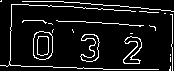
\includegraphics[scale=0.5]{canny.png}
  \caption{Canny算子}
  \label{fig:canny}
\end{figure}

边缘检测算子只能找到所有边缘点,还应从边缘点中找出上下两条横线。本文采用哈夫变换检测这些直线,将其倾斜度作为整个边框的倾斜度。在用OpenCV进行哈夫变换时,需要指定直线的参数$\theta$和$\rho$的量化间隔$\Delta\theta$和$\Delta\rho$。量化间隔太小,计算量过大,并将出现一条边缘线分裂成几条短线的情况;量化间隔太大,检测出的直线不准确。需要反复实验,找出最佳的量化间隔。用多组量化间隔进行哈夫变换,观察结果,最后找出最佳的量化间隔为$\Delta\theta=2^\circ,\Delta\rho=2$。然而,无论如何选取阈值,都无法避免边框断裂成几条直线。因此在计算直线倾斜角时,应该统计多条直线的倾斜角的平均值。求出倾斜度$\theta$后,再将边框图像绕中心按反方向旋转$\theta$角度,使整个边框处于水平位置。旋转后的图像如图\ref{fig:rotate}所示。
\begin{figure}[h]
  \centering
  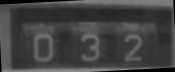
\includegraphics[scale=0.5]{rotate.png}
  \caption{旋转后的图像}
  \label{fig:rotate}
\end{figure}

\section{数字分割}


\subsection{二值化}


分割的第一步是二值化,将数字和背景的像素值设为255和0。观察图\ref{fig:rotate}发现,由于背景部分有反光,数字边框的背景灰度不均匀,不适合使用全局阈值法,应使用局部阈值法对平均灰度不同的小区域取不同的阈值。在局部阈值法的OpenCV实现中,OpenCV提供了两种计算阈值的方式,分别是用盒形滤波模板和高斯滤波模板计算加权平均值作为阈值\upcite{opencvref}。在OpenCV的实现中还可以指定参数$C$,表示将加权平均值加上$C$值作为阈值。因为反光处背景的灰度和数字相差不大,所以邻域内中心像素的权值应高于周围像素,选用高斯滤波模板计算加权平均值。经多次调整参数$C$发现,当$C=1.5$时,即将平均值加上1.5,可以获得较好的二值化图像。此时二值化图像的背景部分还有较多的噪声,数字部分内部有空隙,不利于分割和识别。由\ref{sec:morph}节可知,可以用形态学运算去除噪声并填补空洞。由于数字笔画较细,应先进行闭运算填补空隙,再用开运算减少噪声。为了保证形态学运算后数字的边界基本不变,本文选用的$3\times $十字形的形态学模板,如图\ref{fig:morph}所示。最后得到的二值化图像如图\ref{fig:framebin}所示,可以看出噪声并未完全消除。未消除的噪声需要在后续步骤中进行进一步处理。
\begin{figure}[h]
  \centering
  \includegraphics{cross.eps}
  \caption{形态学模板}
  \label{fig:morph}
\end{figure}

\begin{figure}[h]
  \centering
  
\includegraphics[scale=0.5]{framebin.png}
  \caption{数字边框的二值化图像}
  \label{fig:framebin}
\end{figure}

\subsection{数字定位}\label{sec:charseg}


求出二值化图像后,下一步是找出数字的位置。文献\cite{cookbook}推荐使用连通成分分析进行数字定位。然而,由于本文使用局部阈值法进行二值化,因而在二值化的图像中,数字可能断裂成互不连通的成分,因此不适合使用连通成分分析。综合以上情况,本文使用投影法定位数字。该方法能找出断裂的数字的各个部分。由于电表的数字在滚轮上,数字在竖直方向的位置不一定相同,因此先找出三个数字的在水平方向上各自的范围,然后在三个数字各自的水平范围内的图像做竖直投影。水平方向上的投影如图\ref{fig:projectx}所示。我们称这样的图为\emph{投影直方图}。
\begin{figure}[h]
  \centering
  
\includegraphics[scale=0.5]{projectx.png}
  \caption{水平方向投影}
  \label{fig:projectx}
\end{figure}

比较图\ref{fig:framebin}和\ref{fig:projectx}可得,二值图像的噪声点和线也投影到了横轴上。因此直接从含噪声的投影直方图中找出波峰容易出错。观察噪声对投影直方图的影响可以发现,噪声在投影直方图上形成各处均匀的背景噪声,使直方图整体抬高了。因此,投影直方图的噪声的关键,是找出背景噪声。减去这个幅度,就可以得到不含噪声的直方图。具体做法是,对投影直方图进行排序,找出位于中间处的像素数,作为背景噪声;然后将投影直方图各处均减去背景噪声,得到含噪声的直方图。这样做的理由是,因此在理想的投影直方图中,一半没有任何投影像素,另一半为数字形成的波峰。受背景噪声干扰,没有任何像素的地方都充满了背景噪声。因此,排序的投影直方图的前半部分,只有背景噪声没有数字投影。消除了背景噪声的投影直方图如图\ref{fig:proclear}所示。
\begin{figure}[h]
  \centering
  
\includegraphics[scale=0.5]{proclear.png}
  \caption{消除背景噪声的投影}
  \label{fig:proclear}
\end{figure}

消除了噪声后,下一步是找出数字投影的波峰。观察直方图,可以发现数字的投影往往形成多个尖峰。例如数字“0”两侧的竖直线形成投影直方图的两个尖峰,中间部分形成一个较深的谷底。利用这个特点,我们可以使用类似于滞后阈值的方法找出波峰。具体做法是分别指定一个较高和较低的阈值,用高阈值找出数字投影的尖峰,然后在尖峰的两侧搜索高于低阈值的部分从而找出数字的完整的波峰。然后利用位置、宽度等信息去掉非数字形成的波峰。

用水平投影找出三个数字在水平方向的范围后,再用竖直投影找出三个数字在竖直方向的范围。由于竖直方向的投影只有一个数字,噪声对应的波峰没有数字的宽,因此,只需找出其中最宽的波峰,即可确定竖直方向的方位。经两次投影后,就可以分割出三个数字,如图\ref{fig:digit}所示。
\begin{figure}[h]
  \centering
  
\includegraphics{1.png}\hspace{1cm}
  
\includegraphics{2.png}\hspace{1cm}
  
\includegraphics{3.png}
  \caption{分割出的三个数字}
  \label{fig:digit}
\end{figure}

\section{数字识别}

由于不同电流表的数字形状和大小相同,没有旋转、扭曲、缩放等干扰,因此与前面的过程相比,数字识别是一个较为简单的过程。本文使用模板匹配法进行数字识别,因为模板匹配法具有不需要训练分类器,对数字断裂干扰不敏感等特点,适用于字符较少且字符形状和大小规范的情况。

\subsection{字符归一化}\label{sec:norm}

不同图片分割出的数字大小不一致,笔画粗细也各不相同,位置也有偏差,不利于识别。需要对数字做归一化处理,尽量减小相同数字的多幅图像的差异,进而在相同的标准下进行识别\upcite{vcpattern}。数字归一化的步骤有\emph{位置归一化}、\emph{尺寸归一化}和\emph{笔画粗细归一化}\upcite{vcpattern}。位置归一化的做法是,先计算数字的质心,然后以字符的质心为图像中心,平移图像。尺寸归一化的做法是将较待识别字符的长宽和模板做比较,求出在水平和竖直方向的缩放系数进行缩放运算。笔画粗细归一化相对复杂,因为既要求在尽量细化到笔画只有一个像素宽,又要保证不出现笔画断裂。这是两个矛盾的要求。鉴于待识别的数字形状简单,笔画很少,本文使用Hilditch细化算法\upcite{vcimg}。

Hilditch是简单直观的笔画细化算法,适用于处理二值字符图像,基本原理是逐层减少笔画宽度。为找出外层的笔画像素,Hilditch算法用如图\ref{fig:hilditchmask}所示的$3\times 3$模板判断某个像素是否为外层笔画像素\upcite{vcimg}。
\begin{figure}[h]
  \centering
  \includegraphics{hilditchmask.eps}
  \caption{Hilditch邻域}
  \label{fig:hilditchmask}
\end{figure}
将模板中心和字符像素重合,只有满足如下条件的像素,才判定为外层笔画像素,予以删除\upcite{vcimg}。
\begin{asparaenum}[(1)]

\item $x_1,x_3,x_5,x_7$不全为字符像素;
\item $x_1$到$x_8$不全为背景像素;
\item $x_1$到$x_8$中至少有两个是背景像素;
\end{asparaenum}

Hilditch算法对字符图像进行多轮扫描,每一轮标记待删除的像素,扫描结束后删除标记像素,直到某一轮未标记任何像素。本文的字符图像像素很少,笔画简单,多次扫描的运算量也不大。

\subsection{模板匹配}

不同电流表上的字符大小和形状相同,没有旋转和变形等干扰。数字的黑色背景光照不均匀,导致分割时数字易出现断裂。在这种情况下,适合使用模板匹配法进行数字识别。使用模板匹配法需要制作模板。具体做法是从\ref{sec:charseg}节得到的数字中,找出大小、形状和偏离方向最理想的,按\ref{sec:norm}节的方法统一成$16\times 27$的模板(大部分数字尺寸都在$16\times 27$左右),作为模板。其中,数字“1”不宜使用模板匹配,因为数字“1”比其他数字窄,如果进行归一化,数字“1”的横向拉伸形变非常严重。因此,在模板匹配前,先找出较窄的数字字符图像,通过检测是否为竖直直线确定是否为“1”。

模板匹配的关键是找出待识别数字和模板的差距。这个差距可以用Hausdorff距离度量\upcite{vcimg2}。设$A$是待识别图像的数字部分像素集合,$B$是模板的数字像素的坐标集合,则Hausdorff距离$H(A,B)$定义如下:
\begin{equation}
  \begin{aligned}
    h(A,B)&=\max_{a\in A}\min_{b\in B}||a-b||\\
    h(B,A)&=\max_{b\in B}\min_{a\in A}||a-b||\\
    H(A,B)&=\max(h(A,B),h(B,A))
  \end{aligned}
  \label{eq:hausdorff}
\end{equation}

由式\eqref{eq:hausdorff}可得,计算Hausdorff距离的具体做法是,先找出待识别数字和模板的数字部分的所有像素坐标,然后对于待识别数字的所有坐标,在模板中找出距离最近的坐标,然后取其中最大距离作为两者的Hausdorff距离。取Hausdorff距离最小的模板数字为识别的结果。

\section{实验结果}

为验证本文提出方法的效果,对不同角度不同光照条件下的电流表图像进行了试验。图\ref{fig:meter2}是另一幅电流表图像,图\ref{fig:frame2}是倾斜校正后的数字边框图像,图\ref{fig:digits2}是分割出的三个数字的图像,图\ref{fig:model2}是三个数字的图像分别匹配的三个模板,最终识别结果为036。

\begin{figure}[h]
\centering
  \subfloat[原始图像]{\label{fig:meter2}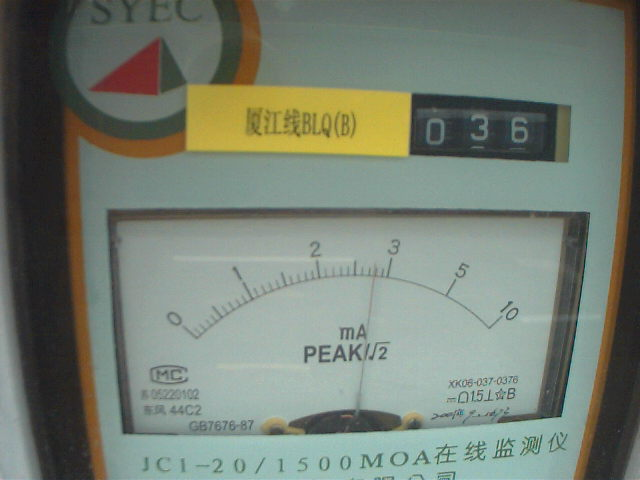
\includegraphics[scale=0.5]{14.png}}\\
\subfloat[数字边框]{\label{fig:frame2}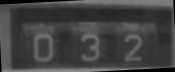
\includegraphics[scale=0.5]{frame2.png}}
\hspace{2cm}
\subfloat[分割的数字]{
  \label{fig:digits2}
  
\includegraphics{digit1.png}\hspace{0.5cm}
  
\includegraphics{digit2.png}\hspace{0.5cm}
  
\includegraphics{digit3.png}}\hspace{2cm}
\subfloat[三个数字模板]{
  \label{fig:model2}
  
\includegraphics{model0.png}\hspace{0.5cm}
  
\includegraphics{model3.png}\hspace{0.5cm}
  
\includegraphics{model6.png}}
\caption{另一张电流表图像的识别过程}
\end{figure}
本文对对47张不同角度不同光照条件下的电流表图像,共141个数字进行了试验。本方法正确识别了其中40张图片共120个数字,识别率为85.1\%。在未正确识别的7张图像中,其中4张是因为数字边框定位不准确,另外2张是因为数字边框图像二值化的效果不理想,最后1张是因为将竖直干扰线误认为数字“1”。影响电流表读数识别率的主要因素有
\begin{inparaenum}[(1)]
\item 电流表的防护玻璃和数字边框的反光较严重;
\item 电流表的防护玻璃灰尘较多;
\item 极少数摄像头未对焦。
\end{inparaenum}
因此,需要在该方法的基础上进行改进,找出更好地减少干扰和噪声的方法,提高识别率。

\section{本章小结}

本章的主要工作是对单个的数字字符图像进行识别。识别的第一步是进行归一化处理,包括位置归一花、尺寸归一化和笔画粗细归一化。然后用数字模板,利用Hausdorff距离衡量待识别像素和模板的差距,选择差距最小的模板对应的数字作为识别结果。该方法简单直观,对本文的电流表图像有较好的识别效果,但仍需要改进,以识别噪声干扰较严重的图像。
%%% Local Variables: 
%%% mode: latex
%%% TeX-master: "thesis"
%%% End: 

%%%
%\CTEXsetup[name={,},number={\arabic{chapter}},format={\zihao{-3}\centering}]{chapter} %正文后面的章标题居然又要改成居中排版。正文用一种样式,文后用另一种,瓜得很。


\chapter{总结与展望}

\section{总结}


由于电流表图像中,与读数无关的部分太多,图像中也含有较多噪声,将读数识别分成图像预处理、数字边框提取、数字分割和数字识别这四个部分。

在预处理部分,为增强图像质量,减少噪声,针对电流表图像的特点,使用了几种常见的图像处理方法。摄像头拍摄的图像是彩色图像,处理比较困难,因此先转换成灰度图像。由于电流表图像采集的时间不同,图像的光照条件也不相同,为了减少光照条件变化带来的影响,使各个时间的图像的灰度大致相同,我们采用直方图均衡化处理图像。然后观察图像噪声的特点,发现主要是孤立的点线噪声。根据噪声的这个特点,本文提出进行高斯滤波以见效噪声。

在数字边框提取部分,首先根据仪表可以分成大片的白色和黑色区域的情况,采用Otsu阈值法,找出黑色区域。然后找出这些像素形成的若干个连通成分。为了减少计算开销,本文逐行扫描算法。然后用连通成分的长宽比、像素密度、像素数目和面积等指标筛选连通成分,找出数字边框对应的连通成分。由于数字边框由一定的倾斜角度,先做水平方向的边缘检测,再利用改进的哈夫变换找出上下两条横线的倾斜角度,然后根据倾斜角度利用仿射变换将数字边框图像旋转回原位置。

在数字分割部分,根据背景不均匀的特点,本文分使用了基于动态阈值的数字分割算法。首先用动态阈值法粗略地找出数字对应的像素,再用形态学的方法填补数字的空洞和缝隙,消除错分为数字像素的背景像素。然后做水平和竖直方向上的投影,通过寻找波峰和波谷,找出数字的位置。

在数字识别部分,本文针对仪表数字大小形状一致和数字分割中易出现断裂和缺口的情况,采用模板匹配法识别数字。在进行模板匹配哦前,需要对待识别图像进行归一化,将数字的尺寸、大小和笔画粗细统一。其中在笔画粗细归一化使用Hilditch算法。最后在匹配模板时,使用Hausdorff距离度量待识别数字和模板的差距,取差距最小的模板对应的数字最为识别结果。

\section{展望}

本文提出了电流表读数识别的算法。在实际应用中,电流表图像的噪声大、干扰多,该算法的准确性和鲁帮性还有待提高。要使上述算法能真正用于电站的电流表自动识别,仍需要做许多细致而深入的工作。

在预处理阶段,部分电流表图像的噪声和干扰比较多,需要使用更有效的图像增强算法。既保证消除噪声和干扰,又不能使待识别的数字模糊。在数字边框定位阶段,Otsu算法对大部分图像都有较好的效果,但对少部分电流表保护玻璃的反光强烈的图像,Otsu算法失效。因此,对于反光强烈的图像,需要使用更有效的算法定位边框。在数字分割阶段,使用局部阈值法得到的二值化图像有许多干扰点线。只有将这些干扰点线几乎全部去除,投影法定位的数字才准确。最后,在数字识别阶段,如何有效地计算数字字符图像和模板的差距,是一个值得考虑的问题。

电流表的自动识别算法可以推广到其他类型仪表的自动识别。然而,各种仪表数字的大小、位置和形状各不相同。如何推广电流表的自动识别算法,找出一般的仪表自动识别的通用规律,也是一个值得探索的问题。
%%% Local Variables: 
%%% mode: latex
%%% TeX-master: "thesis"
%%% End: 
 
%\chapter*{作者在读研期间科研成果介绍}
\begin{thebibliography}{99}\addcontentsline{toc}{chapter}{参考文献}
\bibitem[aaa]{sssssss}
\end{thebibliography}
%%% Local Variables: 
%%% mode: latex
%%% TeX-master: "thesis"
%%% End: 


\chapter*{声\qquad明}\addcontentsline{toc}{chapter}{声明}


本人声明所呈交的学位论文是本人在导师指导下进行的研究工作及取得的研究成果。据我所知,除了文中特别加以标注和致谢的地方外,论文中不包含其他人已经发表或撰写过的研究成果,也不包含为获得四川大学或其他教育机构的学位或证书而使用过的材料。与我一同工作的同志对本研究所做的任何贡献均已在论文中作了明确的说明并表示谢意

本学位论文成果是本人在四川大学读书期间在导师指导下取得的,论文成果归四川大学所有,特此声明。\par
\vspace{60pt}
\begin{flushright}
学位论文作者(签名)\CJKunderline{\hspace*{2in}}\\[24pt]
论文指导教师(签名)\CJKunderline{\hspace*{2in}}\\[24pt]
\today
\end{flushright}


%%% Local Variables: 
%%% mode: latex
%%% TeX-master: "thesis"
%%% End: 


\chapter*{致\qquad谢}\addcontentsline{toc}{chapter}{致谢}

首先感谢Linda Shapiro和George Stockman。他们合著的《计算机视觉》深入浅出地讲述了机器视觉的基本理论和技术。我就是从这本书学到图像处理和计算机视觉的基础知识。另外,Wesley Snyder和Hairong Qi合著的《机器视觉教程》内容浅显,让我在短时间内就掌握了机器视觉的基本算法的要领。刘直芳、王运琼和朱敏老师合编的《数字图像处理与分析》包含了丰富的公式。本文的部分公式就来自这本书。张宏林编著的《Visual C++数字图像模式识别技术与工程实践》和苏彦华编著的《Visual C++数字图像识别技术典型案例》包含了大量的源代码。通过阅读源代码,我实现了自己的毕业设计。在此对他们提出感谢。

毕业论文和设计里大量使用了OpenCV的函数。感谢OpenCV的开发者Vadim Pisarevsky等人。OpenCV提供了许多常见的图像处理和机器视觉算法,大大降低了我开发图像识别程序的难度。为学习OpenCV,我参考了《Mastering OpenCV with Practical Computer Vision Projects》和《OpenCV Cookbook》两本书。为此,向下面这几位作者致谢:Daniel Lélis Baggio,Shervin Emami,David Millán Escrivá,Khvedchenia Ievgen,Naureen Mahmood,Jason Saragih,Roy Shilkrot,Robert Laganière。

本文是用\XeLaTeX~排版的。\XeLaTeX~由基础排版引擎\XeTeX~和高层格式包\LaTeX~组成,而\XeTeX~排版引擎源于\TeX~。所以这里感谢\XeTeX~的开发者Jonathan Kew,\LaTeX~的开发者Leslie Lamport和\TeX~的开发者Donald Knuth。\XeLaTeX~本身的功能有限,仅仅用它是无法完成论文排版的。因此我使用了大量的\LaTeX的扩展包,其中最重要的是\LaTeX中文排版扩展包ctex,所以这里特别感谢开发和维护ctex的中文\TeX~学会。在使用\LaTeX~的过程中,《\LaTeXe~完全学习手册》给了我极大的帮助。这本书详细地解释了常见的\LaTeX~命令。每当我用\LaTeX排版遇到问题时,在这本书里总能找到解决方案,所以这里特别感谢这本书的作者胡伟。本文的插图是用MetaPost制作的。感谢MetaPost的作者John D. Hobby和Taco Hoekwater。没有他们,用\XeLaTeX排版出精美的毕业论文,是难以想象的。

感谢指导毕业论文的张蕾老师和郭泉师兄。在和郭泉师兄的交流中,我逐渐明白了图像识别系统的原理和常见问题。另外感谢卢晓春老师,她提出了许多有关图像识别的宝贵建议,使我找到了合适的算法。最后感谢父母对我的关怀和支持。
%%% Local Variables: 
%%% mode: latex
%%% TeX-master: "thesis"
%%% End: 

\appendix

\chapter{源代码(模块代码主体部分)}
%定义源代码的排版样式
\lstset{
  tabsize=4,
  frame=none,
  stringstyle=\ttfamily,
  numbers=left,
  numberstyle=\small,
  extendedchars=false,columns=flexible,mathescape=true
  numbersep=-1em
}

meter.cpp节选
\lstinputlisting{src/meter.cpp}
position.cpp节选
\begin{lstlisting}
bool findWheel(Mat &src, Mat &dst)
{
    Mat bin, binInv;
    threshold(src, bin, 60.0, 255.0, THRESH_BINARY | THRESH_OTSU);
    imwrite("otsu.png", bin);
    threshold(src, binInv, 60.0, 255.0, THRESH_BINARY_INV | THRESH_OTSU);
    vector<vector<Point> > contours;
    findContours(binInv, contours, CV_RETR_EXTERNAL, CV_CHAIN_APPROX_NONE);
    int idx = selectContour(contours);

    if (idx < 0)
    {
	return false;
    }

    Rect rect = boundingRect(contours[idx]);
    Mat mask(bin.size(), bin.type(), Scalar(0));
    drawContours(mask, contours, idx, Scalar(255), CV_FILLED);
    Mat left;
    src.copyTo(left, mask);
    Mat rotated = src(rect).clone();

    double slant = slantAngle(contours[idx]);
    Point center;
    center.x = rotated.cols / 2;
    center.y = rotated.rows / 2;
    Mat rot = getRotationMatrix2D(center, slant, 1.0);

    warpAffine(rotated, dst, rot, rotated.size());    
    imwrite("frame.png", rotated);
    imwrite("rotate.png", dst);

    return true;
}
\end{lstlisting}
segment.cpp节选
\begin{lstlisting}
void segment(Mat &src, vector<Mat> &digitVec)
{
    Mat bin;
    adaptiveThreshold(src, bin, 255.0, ADAPTIVE_THRESH_GAUSSIAN_C,
		      THRESH_BINARY, 5, -1.5);
    medianBlur(bin, bin, 3);
    morphologyEx(bin, bin, MORPH_CLOSE, Mat());
    imshow("bin", bin);

    MatND px;
    Mat pxImg;
    projectHor(bin, px, 1);
    drawProject(px, pxImg);
    imwrite("projectx.png", pxImg);
    // imshow("horizontal", pxImg);

    trimPro(px, px);
    histerThresh(px, px, 15, 3);
    drawProject(px, pxImg);
    //imshow("thresh_project", pxImg);

    vector<Vec2i> horPeaks;
    findPeaks(px, horPeaks, 5, 35, 2);

    const char *names[10] = {"1.png", "2.png", "3.png", "4.png", "5.png",
     			    "6.png", "7.png", "8.png", "9.png", "10.png"};
     for (int i = 0; i < horPeaks.size(); i++)
     {
       if (horPeaks[i][0] < 10 || horPeaks[i][1] < 15)
       {
	   continue;
       }
      	Mat candDigit = bin(Range(0, bin.rows),
      			Range(horPeaks[i][0], horPeaks[i][1])).clone();
	cout << horPeaks[i][0] << "\t" << horPeaks[i][1] << endl;
 	MatND py;
     	vector<Vec2i> verPeaks;
     	projectVer(candDigit, py, 1);
     	findPeaks(py, verPeaks, 15, 50, 1);

	if (verPeaks.size() > 0)
	{
	    Mat digit = candDigit(Range(verPeaks[0][0], verPeaks[0][1]),
				  Range(0, candDigit.cols));
	    Rect rect(horPeaks[i][0], verPeaks[0][0], 
		      horPeaks[i][1] - horPeaks[i][0],
		      verPeaks[0][1] - verPeaks[0][0]);
	    rectangle(bin, rect.tl(), rect.br(), Scalar(128), 2);
	    digitVec.push_back(digit);
	}
     }
     imshow("bin", bin);
}
\end{lstlisting}

%%% Local Variables: 
%%% mode: latex
%%% TeX-master: "thesis"
%%% End: 


\chapter{翻译(原文和译文)}

\section*{译文}

\begin{center}
 \Large \textbf{灰度直方图的阈值选择方法}\\[10pt]
\normalsize 大津信行\\[10pt]
\end{center}

\textbf{摘要}\ \textit{本文提出了一种为图像分割而进行的非参数且非监督的自动阈值选择方法。最优阈值是用判决准则选取的。这个判决准则使分离的两类的灰度级差距最大。这个过程非常简单,只利用了灰度直方图的零阶和一阶累计矩。可以直观地将这个方法推广到多阈值分割问题。实验结果证实了该方法的有效性。}

\subsection*{概述}


在图像处理中,选取一个合适的灰度阈值,从背景提取图像是非常重要的。就这个问题,人们已经提出了多种技术。在理想的情况下,在直方图中两个波峰中,有一个又深又陡的波谷。这两个波峰分别代表目标和背景。在这种情况下,直方图的波谷就可以作为阈值。然而,对大多数图像,很难精确地找出波谷。尤其是在波谷较为平坦且充满噪声,或者是在两个波峰的高度相差悬殊的情况下,几乎无法找出波谷。有人提出了一些技术用于克服这些困难。例如波谷锐化技术,它将直方图限制在具有较大导数绝对值的像素处(拉普拉斯或梯度)。还有直方图差分技术,即在直方图灰度差分最大处选择阈值。这些方法都利用了邻域像素(或边缘)以修改直方图,以便于选择阈值。另一类方法直接对灰度图使用参数方法。例如,在均方误差意义上,直方图可以用高斯分布近似描述,因而可以使用统计决策方法。然而,这样的方法需要大量单调,甚至不稳定的计算。不仅如此,在许多情况下,高斯分布不能很好地拟合现实情况。在目前发表的方法中,没有哪一个对阈值的优劣做出估计。因此,建立一个合适的衡量阈值优劣的准则,在这个基础上推导最优阈值,是一个合理的做法。

本文假定,从直方图选择最优阈值时,没有使用先验知识。这种假定在标准图像处理技术中十分重要,而且也是模式识别的非监督分类问题中也是十分必要的。利用判别准则,本文提出了新的方法。该方法直接估计阈值的优劣,自动选择最优化的阈值。

\subsection*{公式}

设给定图像的$L$个灰度级分别用$1,2,\cdots,L$表示。灰度为$i$的像素数为$n_i$,总像素数为$N=n_1+n_2+\cdots+n_L$。为简单起见,假定灰度直方图是归一化的,可以视为一个概率分布:
\begin{equation}
  \label{eq:1}
  p_i=\frac{n_i}{N},\quad p_i\geqslant 0,\sum_{i=1}^Lp_i=1
\end{equation}

现在假定我们用阈值$k$将像素分成$C_0$和$C_1$两类,分别表示背景和目标;$C_0$表示灰度在1到$k$之间的像素,$C_1$表示灰度在$k+1$到$L$之间的像素。这两类的概率分布、平均值可以分别用如下公式表示:
\begin{equation}
  \label{eq:2}
  \omega_0=\sum_{i=1}^kp_i=\omega(k)
\end{equation}

\begin{equation}
  \label{eq:3}
  \omega_1=\sum_{i=k+1}^Lp_i=1-\omega(k)
\end{equation}
和
\begin{equation}
  \label{eq:4}
  \mu_0=\sum_{i=1}^k\frac{ip_i}{\omega_0}=\frac{\mu(k)}{\omega(k)}
\end{equation}

\begin{equation}
  \label{eq:5}
  \mu_1=\sum_{i=k+1}^L\frac{ip_i}{\omega_0}=\frac{\mu_T-\mu(k)}{1-\omega(k)}
\end{equation}
其中
\begin{equation}
  \label{eq:6}
  \omega(k)=\sum_{i=1}^kp_i
\end{equation}
和
\begin{equation}
  \label{eq:7}
  \mu(k)=\sum_{i=1}^kip_i
\end{equation}
分别是直方图的零阶和一阶累计矩。又有
\begin{equation}
  \label{eq:8}
  \mu_T=\mu(L)=\sum_{i=1}^Lip_i
\end{equation}
表示原始图像的整个灰度平均值。我们可以很容易地得出,对任意阈值$k$,都有如下关系成立:
\begin{equation}
  \label{eq:9}
  \omega_0\mu_0+\omega_1\mu_1=\mu_T,\quad\omega_0+\omega_1=1
\end{equation}
两类的方差分别用如下公式表示:
\begin{equation}
  \label{eq:10}
  \sigma_0^2=\sum_{i=1}^k(i-\mu_0)^2\frac{p_i}{\omega_0}
\end{equation}

\begin{equation}
  \label{eq:11}
  \sigma_1^2=\sum_{i=1}^k(i-\mu_1)^2\frac{p_i}{\omega_1}
\end{equation}
上述公式需要计算二阶累计矩。

为了估计阈值$k$的优劣,我们需要引入如下判别准则:
\begin{equation}
  \label{eq:12}
  \lambda=\frac{\sigma_B^2}{\sigma_W^2}\quad
  \kappa=\frac{\sigma_W^2}{\sigma_B^2}\quad
  \eta=\frac{\sigma_B^2}{\sigma_T^2}
\end{equation}
其中
\begin{equation}
  \label{eq:13}
  \sigma_W^2 = \omega_0\sigma_0^2+\omega_1\sigma_1^2\\
\end{equation}

\begin{equation}
  \label{eq:14}
  \begin{aligned}
    \sigma_B^2 &= \omega_0(\mu_0-\mu_T)^2+\omega_1(\mu_1-\mu_T)^2
    &= \omega_0\omega_1(\mu_1-\mu_0)^2
  \end{aligned}
\end{equation}
由\eqref{eq:9}可得,
\begin{equation}
  \label{eq:15}
  \sigma_T^2=\sum_{i=1}^L(i-\mu_T)p_i
\end{equation}
上述公式分别是类内方差,类间方差和总方差。然后分割问题可以简化为找出阈值$k$,使\eqref{eq:12}的目标函数最大化。这是一个最优化问题。

这种分割方法假定分割的两类的灰度有较大差别。换句话说,分割效果最佳的阈值应找出两类的最佳分类。

这个判决准则分别找出使最大化$\lambda,\kappa$和$\eta$的$k$值。然而三者是等价的;例如$\kappa=\lambda+1$,$\eta=\frac{\lambda}{\lambda+1}$,因为以下基本关系对任意$k$成立:
\begin{equation}
  \label{eq:16}
  \sigma_W^2+\sigma_B^2=\sigma_T^2
\end{equation}
注意$\sigma_W^2$和$\sigma_B^2$的值和$k$相关,而$\sigma_T^2$与$k$无关。另外注意$\sigma_W^2$基于二阶统计量(方差),而$\sigma_B^2$基于一阶统计量(均值)。因此,$\eta$是关于$k$的最简单的量化函数。故我们选择$\eta$作为衡量阈值$k$的优劣的准则。

使$\eta$或$\sigma_B^2$最优的阈值$k^*$可以用如下迭代搜索。利用简单的累计矩\eqref{eq:6}和\eqref{eq:7},或用\eqref{eq:2}--\eqref{eq:5}:
\begin{equation}
  \label{eq:17}
  \eta(k)=\frac{\sigma_B^2(k)}{\sigma_T^2}
\end{equation}

\begin{equation}
  \label{eq:18}
  \sigma_B^2=\frac{[\mu_T\omega(k)-\mu(k)]^2}{\omega(k)[1-\omega(k)]}
\end{equation}
因此最优阈值$k^*$为:
\begin{equation}
  \label{eq:19}
  \sigma_B(k^*)=\max_{1\leqslant k\leqslant L}\sigma_B^2(k)
\end{equation}

从问题得知,最优阈值$k$的可以简单地限制在:
\begin{equation*}
  S^*=\{k|\omega_0\omega_1=\omega(k)[1-\omega(k)]>0,\quad
  0<\omega(k)<1
\end{equation*}

我们将它称为灰度阈值的有效范围。从公式\eqref{eq:14}的定义可得,在$k\in S-S^*=\{k|\omega(k)=0\textrm{或}1\}$范围内的$k$,判决函数$\sigma_B^2$(或$\eta$)取最小值零,而在$k\in S^*$范围内,取正数值。因此,最优值一定存在。

\subsubsection*{重要分析}

在前面叙述的方法中,除了选择最优阈值外,还需要分析其他一些重要的方面。

对选择的阈值$k^*$,两类的概率分布分别为\eqref{eq:2}和\eqref{eq:3},分别表示用阈值分割后,这两类像素代表的区域所占整幅图像的百分比。两类的均值\eqref{eq:4}和\eqref{eq:5}当作原始灰度图像的均值估计。

最大值$\eta(k^*)$,或简单地记为$\eta^*$,可用于估计两类之间的差别。这是一个重要的度量方式,因为它对灰度的仿射变换不变(例如,对任意旋转和缩放变换$g_i'=ag_i+b$)。它仅仅取如下范围:
\begin{equation*}
  0\leqslant\eta^*\leqslant 1
\end{equation*}
$\eta$取下确界0,当且仅当图像有单一灰度。$\eta$取上确界1,当且仅当图像仅有两种灰度。

\subsubsection*{推广到多阈值}

将该方法推广到多阈值分割问题是直观的。只需推广判决准则。例如,假设将图像分成三个区域,我们需要求出两个阈值:$1\leqslant k_1<k_2<L$,将图像的所有像素分成在$[1,k_1]$区间的类$C_0$,$[k_1+1,k_2]$区间的类$C_1$和$[k_2+1,L]$区间的类$C_2$。准则函数$\sigma_B^2$(也可以取$\eta$)则可以视为两个变量$k_1$和$k_2$的函数,而最优阈值$k_1^*$和$k_2^*$使$\sigma_B^2$最大:
\begin{equation*}
  \sigma_B^2(k_1^*,k_2*)=\max_{1\leqslant k_1<k_2<L}\sigma_B^2(k_1,k_2)
\end{equation*}

需要指出,类别数越多,阈值越难选择。这是因为判决函数$\sigma_B$是用一维灰度直方图定义的,再多类别分割中意义不大。$\sigma_B$的表达式及其优化过程也变得越來越复杂。然而,对分割成两类和三类的问题,该判决准则是非常简单的,因为几乎所有的实际应用都只是这样的问题。因而简化搜索过程是极其必要的。值得一提的是,上述方法可以将$M$类阈值分割问题,简化为求出$M-1$个离散阈值的问题,而在参数方法中,灰度直方图是用高斯分布近似刻画的,需要$3M-1$个连续参数。

\subsubsection*{实验结果}

多个实验样本如图1--3所示。在这些图像中,(a)和(e)是原始灰度图像;(b)和(f)分别是相应的阈值分割结果;(c)和(g)分别是其灰度直方图(已在选择的阈值处做标记),而准则度量$\eta(k)$与此有关。(d)和(h)是分析结果。原始的灰度图像都是$64\times 64$大小。在图1中,图2和图3(a)和图3(e)中,灰度级别分别是16,64,32和256.(通过将字符叠加到图像中,它们都可以转化成相同的16灰度图像,然而这样它们都会丢失精确的灰度细节)。

图1显示了对同一幅含有打字机体的字母“A”加上不同的干扰和噪声。其中图(a)加上了色带,另一幅是原始图像。图2显示了对纹理应用上述方法的结果,其中的直方图都是典型的困难情绪,如平坦的波谷(c)和单峰直方图(g)。为了合适地现实用阈值分割将图像分割成三类的问题,上述方法也应用到细胞图像中,取得了正确的结果,如图3所示,其中$C_0$表示背景,$C_1$表示细胞质,$C_2$表示细胞核。在图(b)和(f)中,它们分别用(),(=)和(*)表示。

目前,从各种样本获取的大量实验结果显示上述从理论上推导的方法也具有实际意义。

\subsubsection*{目标函数的单峰性}

目标函数$\sigma_B^2(k)$,或等价的判别函数$\eta(k)$,总是平滑和单峰的。这一点可以从图1--2的实验结果得知。这证实了该判决准则的优势,同时说明了方法的稳定性。对单峰性质的严格证明尚未得出。然而,由于本文仅关注最大值,证明可以省略。

\subsection*{结论}

用判决准则分析,本文推导了从灰度直方图中自动选择阈值的方法。 它能简单直观地评估阈值的优劣。如下判决准则选出了最佳阈值。也就是使度量函数$\eta$最大化(或者分出的两类的灰度分离程度)。

本文提出的方法具有阈值选择法的非参数和非监督的特性,同时有如下优势。
\begin{enumerate}[1)]
\item 过程简单;只利用了灰度直方图的零阶和一阶累计矩。
\item 由于本方法的判决准则的特性,很容易直接推广到多阈值分割问题。
\item 自动而稳定地选择最优阈值,不是利用直方图的差分(例如波谷等局部特征),而是积分(例如一个全局特征)选择最佳阈值。
\item 重要的方面可以进一步分析(例如估计类的均值和分离程度等)。
\item 本方法非常通用,它适用于多种非监督识别过程。
\end{enumerate}

该方法的应用不仅仅局限于灰度图像的阈值分割。在非监督分类的场合中,只要某些特征的直方图能区分目标,就可以使用该方法。

考虑到这几点,在多种实际问题中,该方法可以作为最简单和标准的自动阈值选择算法。

\subsection*{致谢}

作者感谢信息科学部的主管西野博士,感谢他的款待和鼓励。以及图像处理所所长森喜郎博士,感谢他提供的因为字符和纹理数据,以及有价值的讨论。还有野口博士提供的细胞数据。最后,作者对东京大学的阿玛尼博士表示感谢。

%英文原文使用英文标题样式
\CTEXsetup[name={,},number={\arabic{chapter}},format={\zihao{-3}\centering},beforeskip={-35pt},afterskip={15pt plus 2pt minus 2pt}]{chapter}
\CTEXsetup[format={\zihao{4}\bf\centering}]{section}
\CTEXsetup[format={\zihao{-4}\bf\flushleft}]{subsection}
\CTEXsetup[format={\zihao{-4}\bf\flushleft}]{subsubsection}

\section*{原文}

\begin{center}
 \Large \textbf{A Threshold Selection Method from \\ Gray-Level Histograms}\\[10pt]
\normalsize NOBUYUKI OTSU\\[10pt]
\end{center}

\textit{Abstract}---\textbf{A nonparametric and unsupervised method of automatic threshold selection for picture segmentation is presented. Anoptimal threshold is selected by the discriminant criterion, namely,so as to maximize the separability of the resultant classes in gray levels. The procedure is very simple, utilizing only the zeroth- and the first-order cumulative moments of the gray-level histogram. It is straightforward to extend the method to multithreshold problems.Several experimental results are also presented to support the validity of the method.}

\subsection*{introduction}

It is important in picture processing to select an adequate threshold of gray level for extracting objects from their background. A variety of techniques have been proposed in this regard. In an ideal case, the histogram has a deep and sharp valley between two peaks representing objects and background, respectively, so that the threshold can be chosen at the bottom of this valley [1]. However, for most real pictures, it is often difficult to detect the valley bottom precisely, especially in such cases as when the valley is flat and broad, imbued with noise, or when the two peaks are extremely unequal in height, often producing no traceable valley. There have been some techniques proposed in order to overcome these difficulties. They are, for example, the valley sharpening technique [2], which restricts the histogram to the pixels with large absolute values of derivative (Laplacian or gradient), and the difference histogram method [3], which selects the threshold at the gray level with the maximal amount of difference. These utilize information concerning neighboring pixels (or edges) in the original picture to modify the histogram so as to make it useful for thresholding. Another class of methods deals directly with the gray-level histogram by parametric techniques. For example, the histogram is approximated in the least square sense by a sum of Gaussian distributions, and statistical decision procedures are applied [4]. However, such a method requires considerably tedious and sometimes unstable calculations. Moreover, in many cases, the Gaussian distributions turn out to be a meager approximation of the real modes.

In any event, no "goodness" of threshold has been evaluated in most of the methods so far proposed. This would imply that it could be the right way of deriving an optimal thresholding method to establish an appropriate criterion for evaluating the "goodness" of threshold from a more general standpoint. In this correspondence, our discussion will be confined to the elementary case of threshold selection where only the gray-level histogram suffices without other a priori knowledge. It is not only important as a standard technique in picture processing, but also essential for unsupervised decision problems in pattern recognition. A new method is proposed from the viewpoint of discriminant analysis; it directly approaches the feasibility of evaluating the "goodness" of threshold and automatically selecting an optimal threshold.

\subsection*{formulation}


Let the pixels of a given picture be represented in $L$ gray levels $[1,L]$.  The number of pixels at level $i$ is denoted by $n_i$ and the total number of pixels by $N=n_1+n_2+\cdots+n_L$. In order to simplify the discussion, the gray-level histogram is normalized and regarded as a probability distribution:
\begin{equation}
  \label{eq2:1}
  p_i=\frac{n_i}{N},\quad p_i\geqslant 0,\sum_{i=1}^Lp_i=1
\end{equation}

Now suppose that we dichotomize the pixels into two classed $C_0$ and $C_1$(background and objects, or vice versa) by a threshold at level $k$; $C_0$ denotes pixels with levels $[1,k]$, and $C_1$ denotes pixels with levels $[k+1,L]$. Then the probabilities of class occurrence and the class mean levels, respectively, are given by
\begin{equation}
  \label{eq2:2}
  \omega_0=\sum_{i=1}^kp_i=\omega(k)
\end{equation}

\begin{equation}
  \label{eq2:3}
  \omega_1=\sum_{i=k+1}^Lp_i=1-\omega(k)
\end{equation}
and
\begin{equation}
  \label{eq2:4}
  \mu_0=\sum_{i=1}^k\frac{ip_i}{\omega_0}=\frac{\mu(k)}{\omega(k)}
\end{equation}

\begin{equation}
  \label{eq2:5}
  \mu_1=\sum_{i=k+1}^L\frac{ip_i}{\omega_0}=\frac{\mu_T-\mu(k)}{1-\omega(k)}
\end{equation}
where
\begin{equation}
  \label{eq2:6}
  \omega(k)=\sum_{i=1}^kp_i
\end{equation}
and
\begin{equation}
  \label{eq2:7}
  \mu(k)=\sum_{i=1}^kip_i
\end{equation}
are the zeroth and the first-order cumulative moments of the histogram up to the $k$th level, respectively, and
\begin{equation}
  \label{eq2:8}
  \mu_T=\mu(L)=\sum_{i=1}^Lip_i
\end{equation}
is the total mean level of the original picture. We can easily verify the following relation for any choice of $k$:
\begin{equation}
  \label{eq2:9}
  \omega_0\mu_0+\omega_1\mu_1=\mu_T,\quad\omega_0+\omega_1=1
\end{equation}
The class variances are given by
\begin{equation}
  \label{eq2:10}
  \sigma_0^2=\sum_{i=1}^k(i-\mu_0)^2\frac{p_i}{\omega_0}
\end{equation}

\begin{equation}
  \label{eq2:11}
  \sigma_1^2=\sum_{i=1}^k(i-\mu_1)^2\frac{p_i}{\omega_1}
\end{equation}
These require second-order cumulative moments (statistics). In order to evaluate the "goodness" of the threshold (at level $k$), we shall introduce the following discriminant criterion measures(or measures of class separability) used in the discriminant analysis:
\begin{equation}
  \label{eq2:12}
  \lambda=\frac{\sigma_B^2}{\sigma_W^2}\quad
  \kappa=\frac{\sigma_W^2}{\sigma_B^2}\quad
  \eta=\frac{\sigma_B^2}{\sigma_T^2}
\end{equation}
where
\begin{equation}
  \label{eq2:13}
  \sigma_W^2 = \omega_0\sigma_0^2+\omega_1\sigma_1^2\\
\end{equation}

\begin{equation}
  \label{eq2:14}
  \begin{aligned}
    \sigma_B^2 &= \omega_0(\mu_0-\mu_T)^2+\omega_1(\mu_1-\mu_T)^2
    &= \omega_0\omega_1(\mu_1-\mu_0)^2
  \end{aligned}
\end{equation}
(due to \eqref{eq2:9}) and
\begin{equation}
  \label{eq2:15}
  \sigma_T^2=\sum_{i=1}^L(i-\mu_T)p_i
\end{equation}
are the within-class variance, the between-class variance, and thetotal variance of levels, respectively. Then our problem is reducedto an optimization problem to search for a threshold $k$ that maximizes one of the object functions (the criterion measures) in \eqref{eq2:12}.

this standpoint is motivated by a conjecture that well-thresholded classes would be separated in gray levels, and conersely, a threshold giving the best separation of classes in gray levels would be the best threshold.

The discriminant criteria maximizing $\lambda,\kappa$ and $\eta$, repectively, for $\kappa$ are, however, equivalent to one another; e.g., $\kappa=\eta+1$ and $\eta=\frac{\lambda}{\lambda+1)}$ in terms of $\lambda$, because the following basic relation always holds:
\begin{equation}
  \label{eq2:16}
  \sigma_W^2+\sigma_B^2=\sigma_T^2
\end{equation}

It is noticed that $\sigma_W^2$ and $\sigma_B^2$ are functions of threshold level $k$, but $\sigma_T^2$ is independent of $k$. It is also noted that $\sigma_W^2$ is based on the second-order statistics (class means). Therefor, $\eta$ is the simplese measure with respect to $k$. Thus we adopt $\eta$ as the criterion measure to eveluate the ``goodness''(or separability)of the threshold at level $k$.

The optimal threshold $k^*$ that maximizes $\eta$, or equivalently maximizes $\sigma_B^2$, is selected in the following sequential search by using the simple cumulative quantities \eqref{eq2:6} and \eqref{eq2:7}, or explicitly using \eqref{eq2:2}--\eqref{eq2:5}:
\begin{equation}
  \label{eq2:17}
  \eta(k)=\frac{\sigma_B^2(k)}{\sigma_T^2}
\end{equation}

\begin{equation}
  \label{eq2:18}
  \sigma_B^2=\frac{[\mu_T\omega(k)-\mu(k)]^2}{\omega(k)[1-\omega(k)]}
\end{equation}
and the optimal threshold $k^*$ is 
\begin{equation}
  \label{eq2:19}
  \sigma_B(k^*)=\max_{1\leqslant k\leqslant L}\sigma_B^2(k)
\end{equation}

From the problem, the range of $k$ over which the maximum is sought can be restricted to 
\begin{equation*}
  S^*=\{k|\omega_0\omega_1=\omega(k)[1-\omega(k)]>0,\quad
  0<\omega(k)<1
\end{equation*}
We shall call it the effective range of the gray-level histogram. From the definition in \eqref{eq2:14}, the criterion measure $\sigma_B^2$(or $\eta$) taks a minimum of value of zero for such $k$ as $k\in S-S^*$. It is, therefore, obvious that the maximum always exists.

\subsubsection*{Analysis of further important aspects}

The method proposed in the foregoing affords further means toanalyze iportant aspects other than selecting optimal thresholds.

For the selected threshold $k^*$, the class probabilities \eqref{eq2:2} and \eqref{eq2:3}, respectively, indicate the portions of the areas occupied by the classes in the picture so thresholded. The class means \eqref{eq2:4} and \eqref{eq2:5} serve as estimaates of the mean levels of the classes in the original gray-level picture. 

The maximum value $\eta(k^*)$, denoted simply by $\eta^*$, can be used as a measure to evaluate the separability of classes(or ease of thresholding) for the original picture or the bimodality of the histo-
gram. This is a significant measure, for it is invariant under affine
transformations of the gray-level scale (i.e., for any shift and dila-
tation, $g'_i=ag_i+b$). It is uniquely determined within the range.
\begin{equation*}
  0\leqslant\eta^*\leqslant 1
\end{equation*}
The lower bound (zero) is attainable by, and only by, pictures having a single constant gray level, and the upper bound (unity) is attainable by, and only by, two-valued pictures.

\subsubsection*{Extension to Multithresholding}

The extension of the method to multihresholding problems is straightforward by virtue of the discriminant criterion. For example, in the case of three-thresholding, we assume two thresholds: $1\leqslant k_1<k_2<L$, for separating three classes, $C_0$ for $[1,\cdots,k_1]$, $C_1$ for $[k_1+1,\cdots,k_2]$, and $C_2$ for $[k_2+1,\cdots,L]$. The criterion measure $\sigma_B^2$(also $\eta$) is then a function of two variables $k_1$ and $k_2$, and an optimal set of thresholds $k_1^*$ and $k_2^*$ is selected by maximizing $\sigma_B^2$:
\begin{equation*}
  \sigma_B^2(k_1^*,k_2*)=\max_{1\leqslant k_1<k_2<L}\sigma_B^2(k_1,k_2)
\end{equation*}

It should be noticed that the selected thresholds generally become less credible as the number of classes to be separated increases. This is because the criterion measure ($\sigma_B^2$), defined in one-dimensional(gray-level) scale, may gradually lose its meaning as the number of classes increases. The expression of $\sigma_B^2$ and the maximization procedure also become more and more complicated. However, they are very simple for $M=2$ and 3, which cover almost all practical applications, so that a special method to reduce the search processes is hardly needed. It should be remarked that the parameters required in the present method for $M$-thresholding are $M-1$ discrete thresholds themselves, while the parametric method, where the gray-level histogram is approximated by the sum of Gaussian distributions, requires $3M-1$ continuous parameters.

\subsubsection*{Experimental Results}

Several examples of experimental results are shown in Figs. 1-3. Throughout these figures, (a) (as also (e)) is an original gray-level picture; (b) (and (f)) is the result of thresholding; (c) (and (g)) is a set of the gray-level histogram (marked at the selected threshold) and the criterion measure q1(k) related thereto; and (d) (and (h)) is the result obtained by the analysis. The original gray-level pictures are all 64 x 64 in size, and the numbers of gray levels are 16 in Fig. 1, 64 in Fig. 2, 32 in Fig. 3(a), and 256 in Fig. 3(e). (They all had equal outputs in 16 gray levels by superposition of symbols by reason of representation, so that they may be slightly lacking in precise detail in the gray levels.) Fig. 1 shows the results of the application to an identical character "A" typewritten in different ways, one with a new ribbon (a) and another with an old one (e), respectively. In Fig. 2, the results are shown for textures, where the histograms typically show the difficult cases of a broad and flat valley (c) and a unimodal peak (g). In order to appropriately illustrate the case of three-thresholding, the method has also been applied to cell images with successful results, shown in Fig. 3, where CO stands for the background, C1 for the cytoplasm, and C2 for the nucleus. They are indicated in (b) and (f) by ( ), (=), and (*), respectively.

A number of experimental results so far obtained for various
examples indicate that the present method derived theoretically is
of satisfactory practical use.

\subsubsection*{Unimodality of the object function}

The object function $\sigma_B^2$, or equivalently, the criterion measure $\eta(k)$, is always smooth and unimodal, as can be seen in the experimental results in Figs. 1-2. It may attest to an advantage of the suggested criterion and may also imply the stability of the method. The rigorous proof of the unimodality has not yet been obtained. However, it can be dispensed with from our standpoint concerning only the maximum.

A method to select a threshold automatically from a gray level histogram has been derived from the viewpoint of discriminant analysis. This directly deals with the problem of evaluating the goodness of thresholds. An optimal threshold (or set of thresholds) is selected by the discriminant criterion; namely, by maximizing the discriminant measure $\eta$(or the measure of separability of the resultant classes in gray levels).

The proposed method is characterized by its nonparametric and unsupervised nature of threshold selection and has the following desirable advantages.

\begin{asparaenum}[1)]
\item The procedure is very simple; only the zeroth and the first order cumulative moments of the gray-level histogram are utilized.

\item A straightforward extension to multithresholding problems is feasible by virtue of the criterion on which the method is based.

\item An optimal threshold (or set of thresholds) is selected automatically and stably, not based on the differentiation (i.e.. a local property such as valley), but on the integration (i.e., a global property) of the histogram.

\item Further important aspects can also be analyzed (e.g., estimation of class mean levels, evaluation of class separability, etc.).

\item The method is quite general: it covers a wide scope of unsupervised decision procedure.

\end{asparaenum}

The range of its applications is not restricted only to the thresholding of the gray-level picture, such as specifically described in the foregoing, but it may also cover other cases of unsupervised classification in which a histogram of some characteristic (or feature) discriminative for classifying the objects is available.

Taking into account these points, the method suggested in this correspondence may be recommended as the most simple anid standard one for automatic threshold selection that can be applied to various practical problenms.

\subsection*{Acknowledgement}

The author wishes to thank Dr. H. Nishino, Head of the Information Science Division, for his hospitality and encouragement. Thanks are also due to Dr. S. Mori, Chief of the Picture Processing Section, for the data of characters and textures and valuable discussions, and to Dr. Y. Nogucli for cell data. The author is also very grateful to Professor S. Amari of the University of Tokyo for his cordial and helpful suggestions for revising the presentation of the manuscript.

\subsection*{References}
\newcounter{reference}
\newcommand{\refitem}{\stepcounter{reference}\noindent[\thereference]\quad}

\refitem J. M. S. Prewitt and M. L. Mendelsolhn, "The analysis of cell images," nn.Acad. Sci., vol. 128, pp. 1035-1053, 1966

\refitem J. S. Weszka, R. N. Nagel, and A. Rosenfeld, "A threshold selection technique." IEEE Trans. Comput., vol. C-23, pp. 1322 -1326, 1974

\refitem Watanabe and CYBEST Group. "An automated apparatus for cancer prescreening: CYBEST," Comp. Graph. Imiage Process. vol. 3. pp. 350--358, 1974.

\refitem C. K. Chow and T. Kaneko, "Automatic boundary detection of the left ventricle from cineangiograms," Comput. Biomed. Res., vol. 5, pp. 388- 410, 1972.

\refitem K, Fukunage, Introduction to Statisticul Pattern Recogniition. New York: Academic, 1972, pp. 260-267.


%%% Local Variables:  
%%% mode: latex
%%% TeX-master: "thesis"
%%% End: 

\end{document}

